\documentclass[twoside]{book}

% Packages required by doxygen
\usepackage{fixltx2e}
\usepackage{calc}
\usepackage{doxygen}
\usepackage[export]{adjustbox} % also loads graphicx
\usepackage{graphicx}
\usepackage[utf8]{inputenc}
\usepackage{makeidx}
\usepackage{multicol}
\usepackage{multirow}
\PassOptionsToPackage{warn}{textcomp}
\usepackage{textcomp}
\usepackage[nointegrals]{wasysym}
\usepackage[table]{xcolor}

% Font selection
\usepackage[T1]{fontenc}
\usepackage[scaled=.90]{helvet}
\usepackage{courier}
\usepackage{amssymb}
\usepackage{sectsty}
\renewcommand{\familydefault}{\sfdefault}
\allsectionsfont{%
  \fontseries{bc}\selectfont%
  \color{darkgray}%
}
\renewcommand{\DoxyLabelFont}{%
  \fontseries{bc}\selectfont%
  \color{darkgray}%
}
\newcommand{\+}{\discretionary{\mbox{\scriptsize$\hookleftarrow$}}{}{}}

% Page & text layout
\usepackage{geometry}
\geometry{%
  a4paper,%
  top=2.5cm,%
  bottom=2.5cm,%
  left=2.5cm,%
  right=2.5cm%
}
\tolerance=750
\hfuzz=15pt
\hbadness=750
\setlength{\emergencystretch}{15pt}
\setlength{\parindent}{0cm}
\setlength{\parskip}{3ex plus 2ex minus 2ex}
\makeatletter
\renewcommand{\paragraph}{%
  \@startsection{paragraph}{4}{0ex}{-1.0ex}{1.0ex}{%
    \normalfont\normalsize\bfseries\SS@parafont%
  }%
}
\renewcommand{\subparagraph}{%
  \@startsection{subparagraph}{5}{0ex}{-1.0ex}{1.0ex}{%
    \normalfont\normalsize\bfseries\SS@subparafont%
  }%
}
\makeatother

% Headers & footers
\usepackage{fancyhdr}
\pagestyle{fancyplain}
\fancyhead[LE]{\fancyplain{}{\bfseries\thepage}}
\fancyhead[CE]{\fancyplain{}{}}
\fancyhead[RE]{\fancyplain{}{\bfseries\leftmark}}
\fancyhead[LO]{\fancyplain{}{\bfseries\rightmark}}
\fancyhead[CO]{\fancyplain{}{}}
\fancyhead[RO]{\fancyplain{}{\bfseries\thepage}}
\fancyfoot[LE]{\fancyplain{}{}}
\fancyfoot[CE]{\fancyplain{}{}}
\fancyfoot[RE]{\fancyplain{}{\bfseries\scriptsize Generated by Doxygen }}
\fancyfoot[LO]{\fancyplain{}{\bfseries\scriptsize Generated by Doxygen }}
\fancyfoot[CO]{\fancyplain{}{}}
\fancyfoot[RO]{\fancyplain{}{}}
\renewcommand{\footrulewidth}{0.4pt}
\renewcommand{\chaptermark}[1]{%
  \markboth{#1}{}%
}
\renewcommand{\sectionmark}[1]{%
  \markright{\thesection\ #1}%
}

% Indices & bibliography
\usepackage{natbib}
\usepackage[titles]{tocloft}
\setcounter{tocdepth}{3}
\setcounter{secnumdepth}{5}
\makeindex

% Hyperlinks (required, but should be loaded last)
\usepackage{ifpdf}
\ifpdf
  \usepackage[pdftex,pagebackref=true]{hyperref}
\else
  \usepackage[ps2pdf,pagebackref=true]{hyperref}
\fi
\hypersetup{%
  colorlinks=true,%
  linkcolor=blue,%
  citecolor=blue,%
  unicode%
}

% Custom commands
\newcommand{\clearemptydoublepage}{%
  \newpage{\pagestyle{empty}\cleardoublepage}%
}

\usepackage{caption}
\captionsetup{labelsep=space,justification=centering,font={bf},singlelinecheck=off,skip=4pt,position=top}

%===== C O N T E N T S =====

\begin{document}

% Titlepage & ToC
\pagenumbering{roman}
\begin{titlepage}
\vspace*{7cm}
\begin{center}%
{\Large Online\+Body\+Schema\+Adaptation \\[1ex]\large 2.\+0 }\\
\vspace*{1cm}
{\large Generated by Doxygen 1.8.11}\\
\end{center}
\end{titlepage}
\clearemptydoublepage
\tableofcontents
\clearemptydoublepage
\pagenumbering{arabic}

%--- Begin generated contents ---
\chapter{Online Body Schema Adaptation \& Markerless eye-\/hand kinematic calibration}
\label{index}\hypertarget{index}{}We propose a markerless hand pose estimation software for the i\+Cub humanoid robot. The agent can calibrate its eye-\/hand kinematic chain without any markers which, from a developmental psychology perspective, can be seen as a body schema adaptation.

\subsection*{Overview\+:}


\begin{DoxyItemize}
\item Repository Organization
\item Dependencies \& how to install
\item Running the Modules
\item References
\end{DoxyItemize}

\subsection*{Repository Organization\+:}

The code is divided into three logical components modules\+:

i) the hand pose estimation (see \hyperlink{group__handPoseEstimation-module}{hand\+Pose\+Estimation-\/module}); ii) the Robot’s Internal Model generator (see \hyperlink{group__internalModel}{internal\+Model}); iii) the likelihood assessment (see \hyperlink{group__likelihoodAssessment}{likelihood\+Assessment});

which are implemented, respectively, at the following repository locations\+:
\begin{DoxyItemize}
\item modules/hand\+Pose\+Estimation\+:
\begin{DoxyItemize}
\item \hyperlink{handPoseEstimationModule_8h}{include/hand\+Pose\+Estimation\+Module.\+h}
\item \hyperlink{handPoseEstimationMain_8cpp}{src/hand\+Pose\+Estimation\+Main.\+cpp}
\item \hyperlink{handPoseEstimationModule_8cpp}{src/hand\+Pose\+Estimation\+Module.\+cpp}
\end{DoxyItemize}
\item modules/internalmodel\+:
\begin{DoxyItemize}
\item icub-\/internalmodel-\/right\+A-\/cam-\/\+Lisbon.\+exe
\item icub-\/internalmodel-\/left\+A-\/cam-\/\+Lisbon.\+exe
\end{DoxyItemize}
\item modules/likelihod\+Assessment\+:
\begin{DoxyItemize}
\item \hyperlink{Cuda__Gl_8cu_source}{src/\+Cuda\+\_\+\+Gl.\+cu}
\item \hyperlink{likelihood_8cpp}{src/likelihood.\+cpp}
\end{DoxyItemize}
\end{DoxyItemize}

The software architecture implementing the proposed eye-\/hand calibration solution can be seen in the following picture\+:

 

\subsection*{How to install}

Please refer to the documentation\+:

\hyperlink{installation}{Installation Guide}

\subsection*{Running the Modules}

Please refer to the documentation\+:

\hyperlink{how_to_use}{How to run the modules}

\subsection*{References}

If you use this code please cite the following reference\+: \begin{DoxyVerb}ARTICLE{ 10.3389/frobt.2016.00007,
AUTHOR={Vicente, Pedro  and  Jamone, Lorenzo  and  Bernardino, Alexandre},
TITLE={Online body schema adaptation based on internal mental simulation and multisensory feedback},
JOURNAL={Frontiers in Robotics and AI},
VOLUME={3},
YEAR={2016},
NUMBER={7},
DOI={10.3389/frobt.2016.00007},
ISSN={2296-9144}
}
\end{DoxyVerb}


The full open-\/access article can be found \href{https://doi.org/10.3389/frobt.2016.00007}{\tt here}

\begin{DoxyAuthor}{Author}
Pedro Vicente \href{mailto:pvicente@isr.tecnico.ulisboa.pt}{\tt pvicente@isr.\+tecnico.\+ulisboa.\+pt} 
\end{DoxyAuthor}
\begin{DoxyCopyright}{Copyright}
Released under the terms of the G\+NU G\+PL v3.\+0. 
\end{DoxyCopyright}

\chapter{How to run the modules}
\label{how_to_use}
How to run the modules guide\hypertarget{how_to_use_internalmodel}{}\section{Running the internal model}\label{how_to_use_internalmodel}
Open a terminal and execute the internal model\+: 
\begin{DoxyCode}
icub-internalmodel-rightA-cam-Lisbon.exe -force-opengl 
\end{DoxyCode}
 The internal model should start showing a high F\+PS value (depending on your machine)\hypertarget{how_to_use_with_dataset}{}\section{Testing with the Dataset}\label{how_to_use_with_dataset}
Open a yarpdataplayer 
\begin{DoxyCode}
yarpdataplayer 
\end{DoxyCode}
 and choose the root folder of the \href{https://github.com/vicentepedro/eyeHandCalibrationDataset-Sim}{\tt dataset}.

Open a yarpmanager 
\begin{DoxyCode}
yarpmanager 
\end{DoxyCode}
 and open the X\+ML file\+: 
\begin{DoxyCode}
app/scripts/OnlineBodySchemaAdaptation-dataset.xml 
\end{DoxyCode}
 N\+O\+TE\+: If you do not have I\+C\+U\+B\+Contrib or a make install, the hand\+Pose\+Estimation will not be found by yarpmanager, you can run it on a terminal on the respective build/bin folder.

You should have a yarpmanager similar to this\+:



Push the run button {\bfseries  (1) } . (and the three modules should appear green)

Connected the ports {\bfseries  (2) }.

Open a terminal and type\+: 
\begin{DoxyCode}
yarp rpc /hpe/rpc:i 
\end{DoxyCode}
 {\bfseries Then}, you can type 
\begin{DoxyCode}
help 
\end{DoxyCode}
 to see the options available, but the most important command is\+: 
\begin{DoxyCode}
start 
\end{DoxyCode}
 and the superimposed fingertips will appear on the two yarpviews.\hypertarget{how_to_use_without_dataset}{}\section{Testing with another robot}\label{how_to_use_without_dataset}
Edit the template\+: 
\begin{DoxyCode}
OnlineBodySchemaAdaptation.xml.template
\end{DoxyCode}
 in particular the connection between the both left and right cameras and the head and arm encoders. Open the X\+ML with yarpmanager 
\begin{DoxyCode}
yarpmanager 
\end{DoxyCode}
 After running the modules and connecting the ports, follow the same procedure has the testing with the Dataset section.

\begin{DoxyAuthor}{Author}
Pedro Vicente \href{mailto:pvicente@isr.tecnico.ulisboa.pt}{\tt pvicente@isr.\+tecnico.\+ulisboa.\+pt} ~\newline
 
\end{DoxyAuthor}
\begin{DoxyCopyright}{Copyright}
Released under the terms of the G\+NU G\+PL v3.\+0. 
\end{DoxyCopyright}

\chapter{Installation Guide}
\label{installation}
Step-\/by-\/\+Step Installation Guide\hypertarget{installation_handpose_sec}{}\section{Hand\+Pose\+Estimation}\label{installation_handpose_sec}
{\bfseries Check} its dependencies before installing this module\+:


\begin{DoxyItemize}
\item Y\+A\+RP
\item Open\+CV (tested with v2.\+10 and v3.\+3)
\end{DoxyItemize}

{\bfseries Optional} 
\begin{DoxyItemize}
\item I\+C\+U\+Bcontrib \href{https://github.com/robotology/icub-contrib-common}{\tt link}
\end{DoxyItemize}

{\bfseries Then\+:} 

Open a terminal.

Go to the hand\+Pose\+Estimation module root folder\+:


\begin{DoxyItemize}
\item /\+Online-\/\+Body-\/\+Schema-\/\+Adaptation/modules/hand\+Pose\+Estimation
\end{DoxyItemize}


\begin{DoxyCode}
mkdir build && cd build 
\end{DoxyCode}



\begin{DoxyCode}
ccmake .. 
\end{DoxyCode}


Press {\itshape c} (twice) and, if no error occurs, press {\itshape g} do generate.

Compile the code\+: 
\begin{DoxyCode}
make 
\end{DoxyCode}
 and if you have the I\+C\+U\+Bcontrib repository installed do a 
\begin{DoxyCode}
make install 
\end{DoxyCode}


\begin{DoxyNote}{Note}
The installation process is similar if you are installing this module in a Windows machine)
\end{DoxyNote}
\hypertarget{installation_likelihood_sec}{}\section{Likelihood Assessment}\label{installation_likelihood_sec}
{\bfseries Check} its dependencies before installing this module\+:


\begin{DoxyItemize}
\item Windows Machine
\item Open\+CV (tested with v2.\+10)
\item C\+U\+DA Tool\+Kit (tested with v6.\+5)
\item C\+Make-\/\+Gui
\item Visual Studio (tested with V\+S10) or another C++/\+C\+U\+DA compiler
\end{DoxyItemize}

{\bfseries Then\+:} 

Open the cmake-\/gui executable



In the section {\itshape  where is the source code }, insert the path (absolute path)\+: 
\begin{DoxyCode}
/Online-Body-Schema-Adaptation/modules/likelihoodAssessment 
\end{DoxyCode}
 In the section {\itshape  where to build the binaries }, insert the path (absolute path)\+: 
\begin{DoxyCode}
/Online-Body-Schema-Adaptation/modules/likelihoodAssessment/build 
\end{DoxyCode}
 and press the configure button, choosing the {\itshape 32} {\itshape bit} {\itshape version} of your compiler

The variable {\itshape  C\+U\+D\+A\+\_\+\+S\+D\+K\+\_\+\+R\+O\+O\+T\+\_\+\+D\+IR } will appear and should point to 
\begin{DoxyCode}
C:\(\backslash\)ProgramData\(\backslash\)NVIDIA Corporation\(\backslash\)CUDA Samples\(\backslash\)v6.5\(\backslash\)common 
\end{DoxyCode}
 or similar, according to the C\+U\+DA version installed.

Press generate and open the C\+U\+D\+Acompare\+Edge2.\+sln file (which is inside the build folder)

choose {\itshape Release} version, set Cudacompare\+Edge2 as the Startup project, and build the project.

You should have now a {\itshape Cudacompare\+Edge2.\+dll} file inside the {\itshape Release} folder.\hypertarget{installation_internalmode_sec}{}\section{Robot\textquotesingle{}s Internal Model}\label{installation_internalmode_sec}
Compile the Yarp Bindings for C\#\+:

\href{http://www.yarp.it/yarp_swig.html#yarp_swig_windows}{\tt http\+://www.\+yarp.\+it/yarp\+\_\+swig.\+html\#yarp\+\_\+swig\+\_\+windows}

You should have a {\itshape yarp.\+dll} file after installing the bindings.

Copy the {\itshape Cudacompare\+Edge2.\+dll} file (generated during the compilation of the likelihood Assessment) and the {\itshape yarp.\+dll} to\+: 
\begin{DoxyCode}
modules/internalmodel/icub-internalmodel-rightA-cam-Lisbon\_Data/Plugins/ 
\end{DoxyCode}


\begin{DoxyAuthor}{Author}
Pedro Vicente \href{mailto:pvicente@isr.tecnico.ulisboa.pt}{\tt pvicente@isr.\+tecnico.\+ulisboa.\+pt} ~\newline

\end{DoxyAuthor}
\begin{DoxyCopyright}{Copyright}
Released under the terms of the G\+NU G\+PL v3.\+0. 
\end{DoxyCopyright}

\chapter{Module Index}
\section{Modules}
Here is a list of all modules\+:\begin{DoxyCompactList}
\item \contentsline{section}{likelihood\+Assessment}{\pageref{group__likelihoodAssessment}}{}
\item \contentsline{section}{internal\+Model}{\pageref{group__internalModel}}{}
\item \contentsline{section}{hand\+Pose\+Estimation-\/module}{\pageref{group__handPoseEstimation-module}}{}
\end{DoxyCompactList}

\chapter{Hierarchical Index}
\section{Class Hierarchy}
This inheritance list is sorted roughly, but not completely, alphabetically\+:\begin{DoxyCompactList}
\item \contentsline{section}{hand\+Pose\+Estimation\+\_\+\+I\+DL}{\pageref{classhandPoseEstimation__IDL}}{}
\begin{DoxyCompactList}
\item \contentsline{section}{hand\+Pose\+Estimation\+Module}{\pageref{classhandPoseEstimationModule}}{}
\end{DoxyCompactList}
\end{DoxyCompactList}

\chapter{Data Structure Index}
\section{Data Structures}
Here are the data structures with brief descriptions\+:\begin{DoxyCompactList}
\item\contentsline{section}{\hyperlink{classhandPoseEstimation__IDL}{hand\+Pose\+Estimation\+\_\+\+I\+DL} \\*Hand\+Pose\+Estimation\+\_\+\+I\+DL I\+DL Interface to \hyperlink{group__handPoseEstimation-module}{hand\+Pose\+Estimation-\/module} services }{\pageref{classhandPoseEstimation__IDL}}{}
\item\contentsline{section}{\hyperlink{classhandPoseEstimationModule}{hand\+Pose\+Estimation\+Module} \\*Class \hyperlink{classhandPoseEstimationModule}{hand\+Pose\+Estimation\+Module} }{\pageref{classhandPoseEstimationModule}}{}
\end{DoxyCompactList}

\chapter{File Index}
\section{File List}
Here is a list of all documented files with brief descriptions\+:\begin{DoxyCompactList}
\item\contentsline{section}{/home/pvicente/software/robot-\/code/git-\/vicentepedro/\+Online-\/\+Body-\/\+Schema-\/\+Adaptation/modules/hand\+Pose\+Estimation/include/{\bfseries hand\+Pose\+Estimation\+\_\+\+I\+D\+L.\+h} }{\pageref{handPoseEstimation__IDL_8h}}{}
\item\contentsline{section}{/home/pvicente/software/robot-\/code/git-\/vicentepedro/\+Online-\/\+Body-\/\+Schema-\/\+Adaptation/modules/hand\+Pose\+Estimation/include/\hyperlink{handPoseEstimationModule_8h}{hand\+Pose\+Estimation\+Module.\+h} }{\pageref{handPoseEstimationModule_8h}}{}
\item\contentsline{section}{/home/pvicente/software/robot-\/code/git-\/vicentepedro/\+Online-\/\+Body-\/\+Schema-\/\+Adaptation/modules/hand\+Pose\+Estimation/src/{\bfseries hand\+Pose\+Estimation\+\_\+\+I\+D\+L.\+cpp} }{\pageref{handPoseEstimation__IDL_8cpp}}{}
\item\contentsline{section}{/home/pvicente/software/robot-\/code/git-\/vicentepedro/\+Online-\/\+Body-\/\+Schema-\/\+Adaptation/modules/hand\+Pose\+Estimation/src/\hyperlink{handPoseEstimationMain_8cpp}{hand\+Pose\+Estimation\+Main.\+cpp} }{\pageref{handPoseEstimationMain_8cpp}}{}
\item\contentsline{section}{/home/pvicente/software/robot-\/code/git-\/vicentepedro/\+Online-\/\+Body-\/\+Schema-\/\+Adaptation/modules/hand\+Pose\+Estimation/src/\hyperlink{handPoseEstimationModule_8cpp}{hand\+Pose\+Estimation\+Module.\+cpp} }{\pageref{handPoseEstimationModule_8cpp}}{}
\item\contentsline{section}{/home/pvicente/software/robot-\/code/git-\/vicentepedro/\+Online-\/\+Body-\/\+Schema-\/\+Adaptation/modules/likelihood\+Assessment/src/{\bfseries Cuda\+\_\+\+Gl.\+cu} }{\pageref{Cuda__Gl_8cu}}{}
\item\contentsline{section}{/home/pvicente/software/robot-\/code/git-\/vicentepedro/\+Online-\/\+Body-\/\+Schema-\/\+Adaptation/modules/likelihood\+Assessment/src/\hyperlink{likelihood_8cpp}{likelihood.\+cpp} \\*Class likelihood\+Assessment }{\pageref{likelihood_8cpp}}{}
\end{DoxyCompactList}

\chapter{Module Documentation}
\section{likelihood\+Assessment}
\label{group__likelihoodAssessment}\index{likelihood\+Assessment@{likelihood\+Assessment}}


likelihood Assessment based on edge extraction for the i\+Cub Humanoid Robot Version\+: v2.\+0  


likelihood Assessment based on edge extraction for the i\+Cub Humanoid Robot Version\+: v2.\+0 

\hypertarget{group__internalModel_Description}{}\subsection{Description}\label{group__internalModel_Description}
The likelihood Assessment (\hyperlink{likelihood_8cpp}{likelihood.\+cpp} and \hyperlink{Cuda__Gl_8cu_source}{Cuda\+\_\+\+Gl.\+cu} files) will be used calculate the likelihood metric between the perception and the generated hypotheses inside the internal model exploiting the interoperability between the Open\+GL, C\+U\+DA and Open\+CV libraries.\hypertarget{group__likelihoodAssessment_dependencies_sec}{}\subsection{Dependencies}\label{group__likelihoodAssessment_dependencies_sec}
Open\+CV

C\+U\+DA Tool\+Kit

Check the installation guide in \hyperlink{installation}{Installation Guide} to more details.

\begin{DoxyAuthor}{Author}
Pedro Vicente \href{mailto:pvicente@isr.tecnico.ulisboa.pt}{\tt pvicente@isr.\+tecnico.\+ulisboa.\+pt} ~\newline

\end{DoxyAuthor}
\begin{DoxyCopyright}{Copyright}
Released under the terms of the G\+NU G\+PL v3.\+0. 
\end{DoxyCopyright}

\section{internal\+Model}
\label{group__internalModel}\index{internal\+Model@{internal\+Model}}


Internal model generator based on Unity Game Engine.  


Internal model generator based on Unity Game Engine. 

Version\+: v2.\+0\hypertarget{group__internalModel_Description}{}\subsection{Description}\label{group__internalModel_Description}
The Robot\textquotesingle{}s internal model generator receives head and arm encoders along with the real pre-\/processed perception and generates the appearance of the hand and arm on the left and right cameras calling the likelihood D\+LL function to compute the similarity between the each hypothesis (200 samples)\hypertarget{group__internalModel_Dependencies}{}\subsection{Dependencies}\label{group__internalModel_Dependencies}
Open\+CV C\+U\+DA Tool\+Kit Y\+A\+RP C\# bindings\hypertarget{group__internalModel_Input}{}\subsection{Ports}\label{group__internalModel_Input}
/internalmodel/right\+Arm\+:i Receives the arm encoders /internalmodel/head\+:i Receives the head encoders /internalmodel/cam\+:i Receives both left and right image (side-\/by-\/side)\hypertarget{group__internalModel_Output}{}\subsection{Ports}\label{group__internalModel_Output}
/internalmodel/likelihood\+:o Sends the likelihood vector /internalmodel/fingertips\+:o Sends the projection of the fingertips (u,v pixel) on the left camera image

\begin{DoxyAuthor}{Author}
Pedro Vicente \href{mailto:pvicente@isr.tecnico.ulisboa.pt}{\tt pvicente@isr.\+tecnico.\+ulisboa.\+pt} ~\newline

\end{DoxyAuthor}
\begin{DoxyCopyright}{Copyright}
License terms, for example\+: released under the terms of the G\+NU G\+PL v3.\+0 . 
\end{DoxyCopyright}

\section{hand\+Pose\+Estimation-\/module}
\label{group__handPoseEstimation-module}\index{hand\+Pose\+Estimation-\/module@{hand\+Pose\+Estimation-\/module}}


Sequential Monte Carlo parameters estimation for the i\+Cub Humanoid Robot Version\+: v2.\+0.  


Sequential Monte Carlo parameters estimation for the i\+Cub Humanoid Robot Version\+: v2.\+0. 

\begin{DoxyAuthor}{Author}
Pedro Vicente \href{mailto:pvicente@isr.tecnico.ulisboa.pt}{\tt pvicente@isr.\+tecnico.\+ulisboa.\+pt} ~\newline
 
\end{DoxyAuthor}
\begin{DoxyCopyright}{Copyright}
License terms, for example\+: released under the terms of the G\+NU G\+PL v3.\+0 . 
\end{DoxyCopyright}
\hypertarget{group__handPoseEstimation-module_intro_sec}{}\subsection{Description}\label{group__handPoseEstimation-module_intro_sec}
The hand pose estimation module belongs to the online body schema adaptation architecture. This module generates several samples (particles) to compared with the real images received from the robot. The new particles are generated according to the likelihood received from the internal model after rendering hallucinated images for the right and left images according to the proprioception and estimated angular offsets.\hypertarget{group__handPoseEstimation-module_parameters_sec}{}\subsection{Parameters}\label{group__handPoseEstimation-module_parameters_sec}

\begin{DoxyItemize}
\item --name\+: Name of the module (default=\textquotesingle{}hpe\textquotesingle{})
\item --arm\+: Arm which the module should connect to. (default=\textquotesingle{}right\textquotesingle{})
\item --initial\+Mean\+: Mean for the initial distribution of the particles \mbox{[}in degrees\mbox{]}. (default=0.\+0)
\item --initial\+Std\+Dev\+: Standard Deviation of the initial distribution of the particles \mbox{[}in degrees\mbox{]}. (default=3.\+5)
\item --artificial\+Noise\+Std\+Dev\+: Initial (standard deviation of) Artificial Noise to spread the particles after each iteration \mbox{[}in degrees\mbox{]}. (default=3.\+0)
\item --lower\+Bound\+: Artificial Noise lower bound (Std\+Dev). Should be greater than Zero to prevent the particles to collapse in one simples value \mbox{[}in degrees\mbox{]}. (default=0.\+04)
\item --upper\+Bound\+: Artificial Noise upper bound (Std\+Dev). The artificial noise should have a upper bound to prevent the particles to diverge after each resampling stage (default=3.\+5)
\item --minimum\+Likelihood\+: Minimum\+Likelihood \mbox{[}0,1\mbox{]} in order to resample the particles (default=0.\+55)
\item --increase\+Multiplier\+: increase the artificial noise of a certain value (current\+Value$\ast$increase\+Multiplier) if the maximum likihood is lower than the minimum\+Likelihood (default=1.\+15)
\item --decrease\+Multiplier\+: decrease the artificial noise of a certain value (current\+Value$\ast$decrease\+Multiplier) if the maximum likihood is greater than the minimum\+Likelihood (default=0.\+85)
\item --K\+D\+E\+Std\+Dev\+: Standard deviation of each kernel in the Kernel Density Estimation algorithm \mbox{[}in degrees\mbox{]}. (default=1.\+0)
\item --min\+Iteration\+: number of iterations before output estimated Offsets (default=35) 
\end{DoxyItemize}\hypertarget{group__handPoseEstimation-module_inputports_sec}{}\subsection{Input Ports}\label{group__handPoseEstimation-module_inputports_sec}

\begin{DoxyItemize}
\item /hpe/right\+Cam\+:i \mbox{[}image\mbox{]} \mbox{[}default carrier\+:udp\mbox{]}\+: This port should receive the right image
\item /hpe/left\+Cam\+:i \mbox{[}image\mbox{]} \mbox{[}default carrier\+:udp\mbox{]}\+: This port should receive the left image
\item /hpe/right\+Arm\+:i \mbox{[}Bottle\mbox{]} \mbox{[}default carrier\+:udp\mbox{]}\+: This port should receive the encoders of the right (D\+E\+F\+A\+U\+LT) arm.
\item /hpe/head\+:i \mbox{[}Bottle\mbox{]} \mbox{[}default carrier\+:udp\mbox{]}\+: This port should receive the encoders of the head.
\item /hpe/likelihood\+:i \mbox{[}Bottle\mbox{]} \mbox{[}default carrier\+:udp\mbox{]}\+: This port will receive the likelihood Bottle containing the likelihood for each particles generated in the internal model.
\item /hpe/finger\+Position\+:i \mbox{[}Bottle\mbox{]} \mbox{[}default carrier\+:udp\mbox{]}\+: This port will receive a Bottle containing the fingertips position on the left image for each particles generated in the internal model.
\end{DoxyItemize}\hypertarget{group__handPoseEstimation-module_outputports_sec}{}\subsection{Output Ports}\label{group__handPoseEstimation-module_outputports_sec}

\begin{DoxyItemize}
\item /hpe/\+L\+Rimage\+:o \mbox{[}image\mbox{]} \mbox{[}default carrier\+:udp\mbox{]}\+: This port sends the concatenation of the pre-\/processed left and right image to the internal model.
\item /hpe/head\+:o \mbox{[}Bottle\mbox{]} \mbox{[}default carrier\+:udp\mbox{]}\+: This port sends the encoders of the head to the internal model.
\item /hpe/particles\+:o \mbox{[}Bottle\mbox{]} \mbox{[}default carrier\+:udp\mbox{]}\+: This port sends the encoders of the arm + the estimated offsets to be generated by the internal model
\item /hpe/best\+Offsets\+:o \mbox{[}Bottle\mbox{]} \mbox{[}default carrier\+:udp\mbox{]}\+: This port outputs the best set of Offsets after each iteration of the Sequential Monte Carlo parameter estimation algorithm
\item /hpe/image\+Corrected\+:o \mbox{[}image\mbox{]} \mbox{[}default carrier\+:udp\mbox{]}\+: This port sends the left camera image with the fingertips positions superimposed according with the best estimated set of offsets.
\item /hpe/image\+Canonical\+:o \mbox{[}image\mbox{]} \mbox{[}default carrier\+:udp\mbox{]}\+: This port sends the left camera image with the fingertips positions superimposed according with the canonical model (i.\+e. without angular offsets in the arm)
\end{DoxyItemize}\hypertarget{group__handPoseEstimation-module_services_sec}{}\subsection{Services}\label{group__handPoseEstimation-module_services_sec}

\begin{DoxyItemize}
\item /hpe/rpc\+:i \mbox{[}rpc-\/server\mbox{]}\+: service port . This service is described in \hyperlink{classhandPoseEstimation__IDL}{hand\+Pose\+Estimation\+\_\+\+I\+DL} (hand\+Pose\+Estimation.\+thrift) 
\end{DoxyItemize}
\chapter{Data Structure Documentation}
\section{hand\+Pose\+Estimation\+\_\+\+I\+DL Class Reference}
\label{classhandPoseEstimation__IDL}\index{hand\+Pose\+Estimation\+\_\+\+I\+DL@{hand\+Pose\+Estimation\+\_\+\+I\+DL}}


\hyperlink{classhandPoseEstimation__IDL}{hand\+Pose\+Estimation\+\_\+\+I\+DL} I\+DL Interface to \hyperlink{group__handPoseEstimation-module}{hand\+Pose\+Estimation-\/module} services.  




{\ttfamily \#include $<$hand\+Pose\+Estimation\+\_\+\+I\+D\+L.\+h$>$}

Inheritance diagram for hand\+Pose\+Estimation\+\_\+\+I\+DL\+:\begin{figure}[H]
\begin{center}
\leavevmode
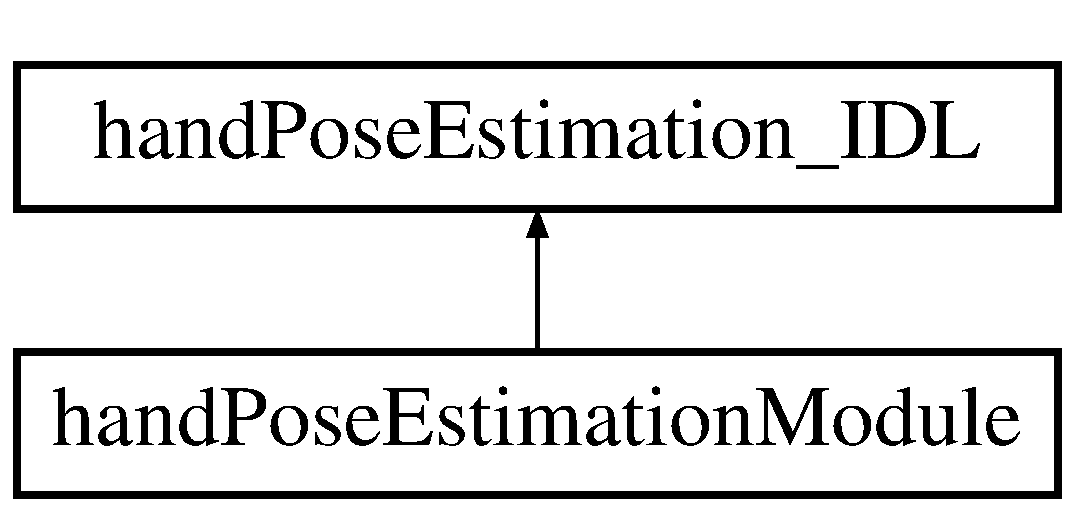
\includegraphics[height=2.000000cm]{classhandPoseEstimation__IDL}
\end{center}
\end{figure}
\subsection*{Public Member Functions}
\begin{DoxyCompactItemize}
\item 
virtual bool \hyperlink{classhandPoseEstimation__IDL_a0168a812d2209bba67212dc2969bc763}{start} ()
\begin{DoxyCompactList}\small\item\em Start (re-\/start) the hand pose estimation. \end{DoxyCompactList}\item 
virtual bool \hyperlink{classhandPoseEstimation__IDL_a9d3f8b39a34db325c89b2c7b44ded1f1}{stop} ()
\begin{DoxyCompactList}\small\item\em Stop the hand pose estimation. \end{DoxyCompactList}\item 
virtual bool \hyperlink{classhandPoseEstimation__IDL_a1f1b82575fb40899ba846bb3afc21406}{pause} ()
\begin{DoxyCompactList}\small\item\em Pause the hand pose estimation. \end{DoxyCompactList}\item 
virtual bool \hyperlink{classhandPoseEstimation__IDL_aea26d5dfb9414ac732c8aee27d4b0bcc}{resume} ()
\begin{DoxyCompactList}\small\item\em Resume the hand pose estimation. \end{DoxyCompactList}\item 
virtual yarp\+::os\+::\+Bottle \hyperlink{classhandPoseEstimation__IDL_a195b385595237044aa81c8a60ec0c75c}{last\+Offsets} ()
\begin{DoxyCompactList}\small\item\em Ask for the last estimated angular Offsets on the arm (7\+DoF) \end{DoxyCompactList}\item 
virtual bool \hyperlink{classhandPoseEstimation__IDL_aeae04edc596badd5c68814d7709c8820}{quit} ()
\begin{DoxyCompactList}\small\item\em Quit the module. \end{DoxyCompactList}\item 
virtual bool {\bfseries read} (yarp\+::os\+::\+Connection\+Reader \&connection) Y\+A\+R\+P\+\_\+\+O\+V\+E\+R\+R\+I\+DE\label{classhandPoseEstimation__IDL_a29990dd4c33d73655d206b0d8e342c83}

\item 
virtual std\+::vector$<$ std\+::string $>$ {\bfseries help} (const std\+::string \&function\+Name=\char`\"{}-\/-\/all\char`\"{})\label{classhandPoseEstimation__IDL_ade8e064ba4c36b3f27c0868c0a7875b8}

\end{DoxyCompactItemize}


\subsection{Detailed Description}
\hyperlink{classhandPoseEstimation__IDL}{hand\+Pose\+Estimation\+\_\+\+I\+DL} I\+DL Interface to \hyperlink{group__handPoseEstimation-module}{hand\+Pose\+Estimation-\/module} services. 

This is a fake thrift service, just to show how to structure your repo and how to document your code. 

Definition at line 20 of file hand\+Pose\+Estimation\+\_\+\+I\+D\+L.\+h.



\subsection{Member Function Documentation}
\index{hand\+Pose\+Estimation\+\_\+\+I\+DL@{hand\+Pose\+Estimation\+\_\+\+I\+DL}!last\+Offsets@{last\+Offsets}}
\index{last\+Offsets@{last\+Offsets}!hand\+Pose\+Estimation\+\_\+\+I\+DL@{hand\+Pose\+Estimation\+\_\+\+I\+DL}}
\subsubsection[{\texorpdfstring{last\+Offsets()}{lastOffsets()}}]{\setlength{\rightskip}{0pt plus 5cm}yarp\+::os\+::\+Bottle hand\+Pose\+Estimation\+\_\+\+I\+D\+L\+::last\+Offsets (
\begin{DoxyParamCaption}
{}
\end{DoxyParamCaption}
)\hspace{0.3cm}{\ttfamily [virtual]}}\label{classhandPoseEstimation__IDL_a195b385595237044aa81c8a60ec0c75c}


Ask for the last estimated angular Offsets on the arm (7\+DoF) 

\begin{DoxyReturn}{Returns}
Bottle with last angular Offsets 
\end{DoxyReturn}


Reimplemented in \hyperlink{classhandPoseEstimationModule_a59ac2a028179a7fbdd6571ef889e3d3b}{hand\+Pose\+Estimation\+Module}.



Definition at line 225 of file hand\+Pose\+Estimation\+\_\+\+I\+D\+L.\+cpp.


\begin{DoxyCode}
225                                                  \{
226   yarp::os::Bottle \_return;
227   handPoseEstimation\_IDL\_lastOffsets helper;
228   helper.init();
229   \textcolor{keywordflow}{if} (!yarp().canWrite()) \{
230     yError(\textcolor{stringliteral}{"Missing server method '%s'?"},\textcolor{stringliteral}{"yarp::os::Bottle handPoseEstimation\_IDL::lastOffsets()"});
231   \}
232   \textcolor{keywordtype}{bool} ok = yarp().write(helper,helper);
233   \textcolor{keywordflow}{return} ok?helper.\_return:\_return;
234 \}
\end{DoxyCode}
\index{hand\+Pose\+Estimation\+\_\+\+I\+DL@{hand\+Pose\+Estimation\+\_\+\+I\+DL}!pause@{pause}}
\index{pause@{pause}!hand\+Pose\+Estimation\+\_\+\+I\+DL@{hand\+Pose\+Estimation\+\_\+\+I\+DL}}
\subsubsection[{\texorpdfstring{pause()}{pause()}}]{\setlength{\rightskip}{0pt plus 5cm}bool hand\+Pose\+Estimation\+\_\+\+I\+D\+L\+::pause (
\begin{DoxyParamCaption}
{}
\end{DoxyParamCaption}
)\hspace{0.3cm}{\ttfamily [virtual]}}\label{classhandPoseEstimation__IDL_a1f1b82575fb40899ba846bb3afc21406}


Pause the hand pose estimation. 

The filter stop the generation of particles and waits for a resume command \begin{DoxyReturn}{Returns}
true/false on success/failure 
\end{DoxyReturn}


Reimplemented in \hyperlink{classhandPoseEstimationModule_ab43685cf6812c7c4c0b1af334f31e94e}{hand\+Pose\+Estimation\+Module}.



Definition at line 205 of file hand\+Pose\+Estimation\+\_\+\+I\+D\+L.\+cpp.


\begin{DoxyCode}
205                                    \{
206   \textcolor{keywordtype}{bool} \_return = \textcolor{keyword}{false};
207   handPoseEstimation\_IDL\_pause helper;
208   helper.init();
209   \textcolor{keywordflow}{if} (!yarp().canWrite()) \{
210     yError(\textcolor{stringliteral}{"Missing server method '%s'?"},\textcolor{stringliteral}{"bool handPoseEstimation\_IDL::pause()"});
211   \}
212   \textcolor{keywordtype}{bool} ok = yarp().write(helper,helper);
213   \textcolor{keywordflow}{return} ok?helper.\_return:\_return;
214 \}
\end{DoxyCode}
\index{hand\+Pose\+Estimation\+\_\+\+I\+DL@{hand\+Pose\+Estimation\+\_\+\+I\+DL}!quit@{quit}}
\index{quit@{quit}!hand\+Pose\+Estimation\+\_\+\+I\+DL@{hand\+Pose\+Estimation\+\_\+\+I\+DL}}
\subsubsection[{\texorpdfstring{quit()}{quit()}}]{\setlength{\rightskip}{0pt plus 5cm}bool hand\+Pose\+Estimation\+\_\+\+I\+D\+L\+::quit (
\begin{DoxyParamCaption}
{}
\end{DoxyParamCaption}
)\hspace{0.3cm}{\ttfamily [virtual]}}\label{classhandPoseEstimation__IDL_aeae04edc596badd5c68814d7709c8820}


Quit the module. 

\begin{DoxyReturn}{Returns}
true/false on success/failure 
\end{DoxyReturn}


Reimplemented in \hyperlink{classhandPoseEstimationModule_a74ab9a34c397b41e805f5124fb8c2bda}{hand\+Pose\+Estimation\+Module}.



Definition at line 235 of file hand\+Pose\+Estimation\+\_\+\+I\+D\+L.\+cpp.


\begin{DoxyCode}
235                                   \{
236   \textcolor{keywordtype}{bool} \_return = \textcolor{keyword}{false};
237   handPoseEstimation\_IDL\_quit helper;
238   helper.init();
239   \textcolor{keywordflow}{if} (!yarp().canWrite()) \{
240     yError(\textcolor{stringliteral}{"Missing server method '%s'?"},\textcolor{stringliteral}{"bool handPoseEstimation\_IDL::quit()"});
241   \}
242   \textcolor{keywordtype}{bool} ok = yarp().write(helper,helper);
243   \textcolor{keywordflow}{return} ok?helper.\_return:\_return;
244 \}
\end{DoxyCode}
\index{hand\+Pose\+Estimation\+\_\+\+I\+DL@{hand\+Pose\+Estimation\+\_\+\+I\+DL}!resume@{resume}}
\index{resume@{resume}!hand\+Pose\+Estimation\+\_\+\+I\+DL@{hand\+Pose\+Estimation\+\_\+\+I\+DL}}
\subsubsection[{\texorpdfstring{resume()}{resume()}}]{\setlength{\rightskip}{0pt plus 5cm}bool hand\+Pose\+Estimation\+\_\+\+I\+D\+L\+::resume (
\begin{DoxyParamCaption}
{}
\end{DoxyParamCaption}
)\hspace{0.3cm}{\ttfamily [virtual]}}\label{classhandPoseEstimation__IDL_aea26d5dfb9414ac732c8aee27d4b0bcc}


Resume the hand pose estimation. 

The filter resumes the generation of particles after a pause command \begin{DoxyReturn}{Returns}
true/false on success/failure 
\end{DoxyReturn}


Reimplemented in \hyperlink{classhandPoseEstimationModule_aebfd952abd71f3faf9270efb2a8c5241}{hand\+Pose\+Estimation\+Module}.



Definition at line 215 of file hand\+Pose\+Estimation\+\_\+\+I\+D\+L.\+cpp.


\begin{DoxyCode}
215                                     \{
216   \textcolor{keywordtype}{bool} \_return = \textcolor{keyword}{false};
217   handPoseEstimation\_IDL\_resume helper;
218   helper.init();
219   \textcolor{keywordflow}{if} (!yarp().canWrite()) \{
220     yError(\textcolor{stringliteral}{"Missing server method '%s'?"},\textcolor{stringliteral}{"bool handPoseEstimation\_IDL::resume()"});
221   \}
222   \textcolor{keywordtype}{bool} ok = yarp().write(helper,helper);
223   \textcolor{keywordflow}{return} ok?helper.\_return:\_return;
224 \}
\end{DoxyCode}
\index{hand\+Pose\+Estimation\+\_\+\+I\+DL@{hand\+Pose\+Estimation\+\_\+\+I\+DL}!start@{start}}
\index{start@{start}!hand\+Pose\+Estimation\+\_\+\+I\+DL@{hand\+Pose\+Estimation\+\_\+\+I\+DL}}
\subsubsection[{\texorpdfstring{start()}{start()}}]{\setlength{\rightskip}{0pt plus 5cm}bool hand\+Pose\+Estimation\+\_\+\+I\+D\+L\+::start (
\begin{DoxyParamCaption}
{}
\end{DoxyParamCaption}
)\hspace{0.3cm}{\ttfamily [virtual]}}\label{classhandPoseEstimation__IDL_a0168a812d2209bba67212dc2969bc763}


Start (re-\/start) the hand pose estimation. 

The filter generates particles and update the particle distribution accordingly \begin{DoxyReturn}{Returns}
true/false on success/failure 
\end{DoxyReturn}


Reimplemented in \hyperlink{classhandPoseEstimationModule_aec7a8ef91db9cfde42966bdf90f50363}{hand\+Pose\+Estimation\+Module}.



Definition at line 185 of file hand\+Pose\+Estimation\+\_\+\+I\+D\+L.\+cpp.


\begin{DoxyCode}
185                                    \{
186   \textcolor{keywordtype}{bool} \_return = \textcolor{keyword}{false};
187   handPoseEstimation\_IDL\_start helper;
188   helper.init();
189   \textcolor{keywordflow}{if} (!yarp().canWrite()) \{
190     yError(\textcolor{stringliteral}{"Missing server method '%s'?"},\textcolor{stringliteral}{"bool handPoseEstimation\_IDL::start()"});
191   \}
192   \textcolor{keywordtype}{bool} ok = yarp().write(helper,helper);
193   \textcolor{keywordflow}{return} ok?helper.\_return:\_return;
194 \}
\end{DoxyCode}
\index{hand\+Pose\+Estimation\+\_\+\+I\+DL@{hand\+Pose\+Estimation\+\_\+\+I\+DL}!stop@{stop}}
\index{stop@{stop}!hand\+Pose\+Estimation\+\_\+\+I\+DL@{hand\+Pose\+Estimation\+\_\+\+I\+DL}}
\subsubsection[{\texorpdfstring{stop()}{stop()}}]{\setlength{\rightskip}{0pt plus 5cm}bool hand\+Pose\+Estimation\+\_\+\+I\+D\+L\+::stop (
\begin{DoxyParamCaption}
{}
\end{DoxyParamCaption}
)\hspace{0.3cm}{\ttfamily [virtual]}}\label{classhandPoseEstimation__IDL_a9d3f8b39a34db325c89b2c7b44ded1f1}


Stop the hand pose estimation. 

The filter stop the generation of particles and waits for a start command \begin{DoxyReturn}{Returns}
true/false on success/failure 
\end{DoxyReturn}


Reimplemented in \hyperlink{classhandPoseEstimationModule_aa742424fe8c42bf74a908ab8eff2b0ab}{hand\+Pose\+Estimation\+Module}.



Definition at line 195 of file hand\+Pose\+Estimation\+\_\+\+I\+D\+L.\+cpp.


\begin{DoxyCode}
195                                   \{
196   \textcolor{keywordtype}{bool} \_return = \textcolor{keyword}{false};
197   handPoseEstimation\_IDL\_stop helper;
198   helper.init();
199   \textcolor{keywordflow}{if} (!yarp().canWrite()) \{
200     yError(\textcolor{stringliteral}{"Missing server method '%s'?"},\textcolor{stringliteral}{"bool handPoseEstimation\_IDL::stop()"});
201   \}
202   \textcolor{keywordtype}{bool} ok = yarp().write(helper,helper);
203   \textcolor{keywordflow}{return} ok?helper.\_return:\_return;
204 \}
\end{DoxyCode}


The documentation for this class was generated from the following files\+:\begin{DoxyCompactItemize}
\item 
/home/pvicente/software/robot-\/code/git-\/vicentepedro/\+Online-\/\+Body-\/\+Schema-\/\+Adaptation/modules/hand\+Pose\+Estimation/include/hand\+Pose\+Estimation\+\_\+\+I\+D\+L.\+h\item 
/home/pvicente/software/robot-\/code/git-\/vicentepedro/\+Online-\/\+Body-\/\+Schema-\/\+Adaptation/modules/hand\+Pose\+Estimation/src/hand\+Pose\+Estimation\+\_\+\+I\+D\+L.\+cpp\end{DoxyCompactItemize}

\section{hand\+Pose\+Estimation\+Module Class Reference}
\label{classhandPoseEstimationModule}\index{hand\+Pose\+Estimation\+Module@{hand\+Pose\+Estimation\+Module}}


Class \hyperlink{classhandPoseEstimationModule}{hand\+Pose\+Estimation\+Module}.  




{\ttfamily \#include $<$hand\+Pose\+Estimation\+Module.\+h$>$}

Inheritance diagram for hand\+Pose\+Estimation\+Module\+:\begin{figure}[H]
\begin{center}
\leavevmode
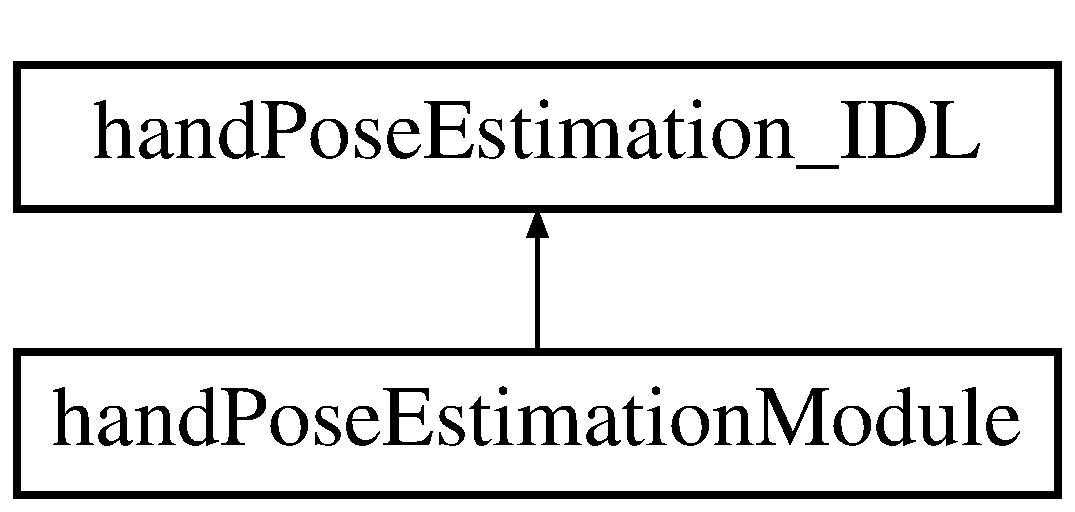
\includegraphics[height=2.000000cm]{classhandPoseEstimationModule}
\end{center}
\end{figure}
\subsection*{Public Member Functions}
\begin{DoxyCompactItemize}
\item 
virtual bool {\bfseries configure} (yarp\+::os\+::\+Resource\+Finder \&rf)\label{classhandPoseEstimationModule_af5197dc0855f11f1acc9c346d8db4983}

\item 
virtual bool {\bfseries interrupt\+Module} ()\label{classhandPoseEstimationModule_a09e731bf904a5b3d87e4c1be6a5faa20}

\item 
virtual bool {\bfseries close} ()\label{classhandPoseEstimationModule_a647af57556f324abb187fe89a2939914}

\item 
virtual bool {\bfseries update\+Module} ()\label{classhandPoseEstimationModule_ae15f1e537aeafdba4c15ae8e8a9aa59a}

\item 
virtual double {\bfseries get\+Period} ()\label{classhandPoseEstimationModule_a8f14212e01137285bd05b3f8a2d8b782}

\item 
bool {\bfseries attach} (yarp\+::os\+::\+Rpc\+Server \&source)\label{classhandPoseEstimationModule_a5f806eba28e4a2a7d36269ffb4a49f7c}

\item 
bool \hyperlink{classhandPoseEstimationModule_aec7a8ef91db9cfde42966bdf90f50363}{start} ()
\begin{DoxyCompactList}\small\item\em Start (re-\/start) the hand pose estimation. \end{DoxyCompactList}\item 
bool \hyperlink{classhandPoseEstimationModule_aa742424fe8c42bf74a908ab8eff2b0ab}{stop} ()
\begin{DoxyCompactList}\small\item\em Stop the hand pose estimation. \end{DoxyCompactList}\item 
bool \hyperlink{classhandPoseEstimationModule_ab43685cf6812c7c4c0b1af334f31e94e}{pause} ()
\begin{DoxyCompactList}\small\item\em Pause the hand pose estimation. \end{DoxyCompactList}\item 
bool \hyperlink{classhandPoseEstimationModule_aebfd952abd71f3faf9270efb2a8c5241}{resume} ()
\begin{DoxyCompactList}\small\item\em Resume the hand pose estimation. \end{DoxyCompactList}\item 
yarp\+::os\+::\+Bottle \hyperlink{classhandPoseEstimationModule_a59ac2a028179a7fbdd6571ef889e3d3b}{last\+Offsets} ()
\begin{DoxyCompactList}\small\item\em Ask for the last estimated angular Offsets on the arm (7\+DoF) \end{DoxyCompactList}\item 
bool \hyperlink{classhandPoseEstimationModule_a74ab9a34c397b41e805f5124fb8c2bda}{quit} ()
\begin{DoxyCompactList}\small\item\em Quit the module. \end{DoxyCompactList}\item 
virtual bool {\bfseries read} (yarp\+::os\+::\+Connection\+Reader \&connection) Y\+A\+R\+P\+\_\+\+O\+V\+E\+R\+R\+I\+DE\label{classhandPoseEstimation__IDL_a29990dd4c33d73655d206b0d8e342c83}

\item 
virtual std\+::vector$<$ std\+::string $>$ {\bfseries help} (const std\+::string \&function\+Name=\char`\"{}-\/-\/all\char`\"{})\label{classhandPoseEstimation__IDL_ade8e064ba4c36b3f27c0868c0a7875b8}

\end{DoxyCompactItemize}
\subsection*{Protected Member Functions}
\begin{DoxyCompactItemize}
\item 
cv\+::\+Mat \hyperlink{classhandPoseEstimationModule_a50367df17ce84fad3013c9d1ad8046ef}{process\+Images} (cv\+::\+Mat input\+Image)
\begin{DoxyCompactList}\small\item\em The function applies a canny edge detector and a distance transform. \end{DoxyCompactList}\item 
bool \hyperlink{classhandPoseEstimationModule_aafbe3332af03ca7e53a8c10f88aa053b}{initialize\+S\+M\+C\+Variables} ()
\begin{DoxyCompactList}\small\item\em Initialize the variables structs needed for the S\+MC to run. \end{DoxyCompactList}\item 
bool \hyperlink{classhandPoseEstimationModule_ad4081c972d64010b87be4ba10a8b967d}{init\+S\+MC} ()
\begin{DoxyCompactList}\small\item\em Initialize the variables values for the S\+MC. \end{DoxyCompactList}\item 
bool \hyperlink{classhandPoseEstimationModule_a05f882cb3c4c6db81ec2e206cd7eb695}{run\+S\+M\+C\+Iteration} ()
\begin{DoxyCompactList}\small\item\em Run one iteration of the Sequential Monte Carlo Parameters estimation. \end{DoxyCompactList}\item 
void \hyperlink{classhandPoseEstimationModule_ab347a264eb373426ecc9e96cf05bafb9}{merge\+And\+Flip\+Images} ()
\begin{DoxyCompactList}\small\item\em merge the left and right images. \end{DoxyCompactList}\item 
void \hyperlink{classhandPoseEstimationModule_ae3b532f8f459b758a8897a4f05dfe704}{kernel\+Density\+Estimation} ()\label{classhandPoseEstimationModule_ae3b532f8f459b758a8897a4f05dfe704}

\begin{DoxyCompactList}\small\item\em Perform the Kernel Density estimation with a multivariate gaussian kernel. \end{DoxyCompactList}\item 
bool \hyperlink{classhandPoseEstimationModule_a4a5ca4a283875fe6af208a0a4e93fd79}{read\+Arm\+Joints} ()
\begin{DoxyCompactList}\small\item\em Read the arm joints. \end{DoxyCompactList}\item 
bool \hyperlink{classhandPoseEstimationModule_a047f05204cd073243f64ac149997d7db}{read\+Head\+Joints} ()
\begin{DoxyCompactList}\small\item\em Read the head joints. \end{DoxyCompactList}\item 
bool \hyperlink{classhandPoseEstimationModule_a9da864a1b3853a9f631b6d3a5caad77d}{systematic\+\_\+resampling} (Cv\+Mat $\ast$old\+Particles\+State, Cv\+Mat $\ast$old\+Particles\+Weights, Cv\+Mat $\ast$new\+Particles\+State, Cv\+Mat $\ast$cum\+Weight, float sum2)
\begin{DoxyCompactList}\small\item\em perform the systematic resampling step of the S\+MC algorithm \end{DoxyCompactList}\end{DoxyCompactItemize}


\subsection{Detailed Description}
Class \hyperlink{classhandPoseEstimationModule}{hand\+Pose\+Estimation\+Module}. 



Definition at line 53 of file hand\+Pose\+Estimation\+Module.\+h.



\subsection{Member Function Documentation}
\index{hand\+Pose\+Estimation\+Module@{hand\+Pose\+Estimation\+Module}!initialize\+S\+M\+C\+Variables@{initialize\+S\+M\+C\+Variables}}
\index{initialize\+S\+M\+C\+Variables@{initialize\+S\+M\+C\+Variables}!hand\+Pose\+Estimation\+Module@{hand\+Pose\+Estimation\+Module}}
\subsubsection[{\texorpdfstring{initialize\+S\+M\+C\+Variables()}{initializeSMCVariables()}}]{\setlength{\rightskip}{0pt plus 5cm}bool hand\+Pose\+Estimation\+Module\+::initialize\+S\+M\+C\+Variables (
\begin{DoxyParamCaption}
{}
\end{DoxyParamCaption}
)\hspace{0.3cm}{\ttfamily [protected]}}\label{classhandPoseEstimationModule_aafbe3332af03ca7e53a8c10f88aa053b}


Initialize the variables structs needed for the S\+MC to run. 

\begin{DoxyReturn}{Returns}
true/false on success/failure 
\end{DoxyReturn}


Definition at line 92 of file hand\+Pose\+Estimation\+Module.\+cpp.


\begin{DoxyCode}
93 \{
94     nParticles=200; \textcolor{comment}{// HardCoded since the Internal Model should be recompiled to support a different
       amount of particles}
95 
96     \textcolor{comment}{//allocate memory for the particles;}
97     particles=cvCreateMat(8,nParticles,CV\_32FC1); \textcolor{comment}{// 0-6 Betas 7- likelihood}
98     \textcolor{comment}{//fill the memory with zeros}
99     cvSetZero(particles);
100 
101     \textcolor{comment}{//define ways of accessing the particles:}
102     \textcolor{comment}{// Beta1}
103     particles1 = cvCreateMatHeader( 1,nParticles, CV\_32FC1);
104     cvInitMatHeader( particles1, 1, nParticles, CV\_32FC1, particles->data.ptr, particles->step );
105     \textcolor{comment}{// Beta2}
106     particles2 = cvCreateMatHeader( 1,nParticles, CV\_32FC1);
107     cvInitMatHeader( particles2, 1, nParticles, CV\_32FC1, particles->data.ptr + particles->step*1, 
      particles->step );
108     \textcolor{comment}{// Beta3}
109     particles3 = cvCreateMatHeader( 1,nParticles, CV\_32FC1);
110     cvInitMatHeader( particles3, 1, nParticles, CV\_32FC1, particles->data.ptr + particles->step*2, 
      particles->step );
111     \textcolor{comment}{// Beta4}
112     particles4 = cvCreateMatHeader( 1,nParticles, CV\_32FC1);
113     cvInitMatHeader( particles4, 1, nParticles, CV\_32FC1, particles->data.ptr + particles->step*3, 
      particles->step );
114     \textcolor{comment}{// Beta5}
115     particles5 = cvCreateMatHeader( 1,nParticles, CV\_32FC1);
116     cvInitMatHeader( particles5, 1, nParticles, CV\_32FC1, particles->data.ptr + particles->step*4, 
      particles->step );
117     \textcolor{comment}{// Beta6}
118     particles6 = cvCreateMatHeader( 1,nParticles, CV\_32FC1);
119     cvInitMatHeader( particles6, 1, nParticles, CV\_32FC1, particles->data.ptr + particles->step*5, 
      particles->step );
120     \textcolor{comment}{// Beta7}
121     particles7 = cvCreateMatHeader( 1,nParticles, CV\_32FC1);
122     cvInitMatHeader( particles7, 1, nParticles, CV\_32FC1, particles->data.ptr + particles->step*6, 
      particles->step );
123     \textcolor{comment}{// likelihood}
124     particles8 = cvCreateMatHeader( 1,nParticles, CV\_32FC1);
125     cvInitMatHeader( particles8, 1, nParticles, CV\_32FC1, particles->data.ptr + particles->step*7, 
      particles->step );
126 
127     \textcolor{comment}{//theta1-theta7}
128     particles1to7 = cvCreateMatHeader( 7,nParticles, CV\_32FC1);
129     cvInitMatHeader( particles1to7, 7, nParticles, CV\_32FC1, particles->data.ptr, particles->step );
130 
131 
132     newParticles=cvCreateMat(8,nParticles,CV\_32FC1);
133     newParticles1to7 = cvCreateMatHeader( 7,nParticles, CV\_32FC1);
134     cvInitMatHeader( newParticles1to7, 7, nParticles, CV\_32FC1, newParticles->data.ptr, newParticles->step 
      );
135     \textcolor{comment}{// Resampling stuff}
136     cumWeight =cvCreateMat(1,nParticles+1,CV\_32FC1);
137     noise=cvCreateMat(7,nParticles,CV\_32FC1);
138     cvSetZero(noise);   
139     \textcolor{keywordflow}{return} \textcolor{keyword}{true};
140 \}
\end{DoxyCode}
\index{hand\+Pose\+Estimation\+Module@{hand\+Pose\+Estimation\+Module}!init\+S\+MC@{init\+S\+MC}}
\index{init\+S\+MC@{init\+S\+MC}!hand\+Pose\+Estimation\+Module@{hand\+Pose\+Estimation\+Module}}
\subsubsection[{\texorpdfstring{init\+S\+M\+C()}{initSMC()}}]{\setlength{\rightskip}{0pt plus 5cm}bool hand\+Pose\+Estimation\+Module\+::init\+S\+MC (
\begin{DoxyParamCaption}
{}
\end{DoxyParamCaption}
)\hspace{0.3cm}{\ttfamily [protected]}}\label{classhandPoseEstimationModule_ad4081c972d64010b87be4ba10a8b967d}


Initialize the variables values for the S\+MC. 

\begin{DoxyReturn}{Returns}
true/false on success/failure 
\end{DoxyReturn}


Definition at line 142 of file hand\+Pose\+Estimation\+Module.\+cpp.


\begin{DoxyCode}
143 \{
144     \textcolor{comment}{// Generate random particles}
145 
146     srand((\textcolor{keywordtype}{unsigned} \textcolor{keywordtype}{int})time(0)); \textcolor{comment}{//make sure random numbers are really random.}
147     rngState = cvRNG(rand());
148 
149     cvRandArr( &rngState, particles1, CV\_RAND\_NORMAL, cvScalar(initialMean), cvScalar(initialStdDev));
150     \textcolor{comment}{//initialize Theta2}
151     cvRandArr( &rngState, particles2, CV\_RAND\_NORMAL, cvScalar(initialMean), cvScalar(initialStdDev));
152     \textcolor{comment}{//initialize Theta3}
153     cvRandArr( &rngState, particles3, CV\_RAND\_NORMAL, cvScalar(initialMean), cvScalar(initialStdDev));
154     \textcolor{comment}{//initialize Theta4}
155     cvRandArr( &rngState, particles4, CV\_RAND\_NORMAL, cvScalar(initialMean), cvScalar(initialStdDev));
156     \textcolor{comment}{//initialize Theta5}
157     cvRandArr( &rngState, particles5, CV\_RAND\_NORMAL, cvScalar(initialMean), cvScalar(initialStdDev));
158     \textcolor{comment}{//initialize Theta6}
159     cvRandArr( &rngState, particles6, CV\_RAND\_NORMAL, cvScalar(initialMean), cvScalar(initialStdDev));
160     \textcolor{comment}{//initialize Theta7}
161     cvRandArr( &rngState, particles7, CV\_RAND\_NORMAL, cvScalar(initialMean), cvScalar(initialStdDev));
162 
163     \textcolor{comment}{// Artificial Noise Initialization}
164     artifNoiseStdDev = initialArtificialNoiseStdDev;
165     \textcolor{comment}{// Setting first particle as Zero offset    }
166     \textcolor{keywordflow}{for} (\textcolor{keywordtype}{unsigned} \textcolor{keywordtype}{int} joint=0;joint<8;joint++) 
167     \{
168         cvmSet(particles,joint,0,0.0);
169     \}
170     \textcolor{keywordflow}{return} \textcolor{keyword}{true};
171 \}
\end{DoxyCode}
\index{hand\+Pose\+Estimation\+Module@{hand\+Pose\+Estimation\+Module}!last\+Offsets@{last\+Offsets}}
\index{last\+Offsets@{last\+Offsets}!hand\+Pose\+Estimation\+Module@{hand\+Pose\+Estimation\+Module}}
\subsubsection[{\texorpdfstring{last\+Offsets()}{lastOffsets()}}]{\setlength{\rightskip}{0pt plus 5cm}yarp\+::os\+::\+Bottle hand\+Pose\+Estimation\+Module\+::last\+Offsets (
\begin{DoxyParamCaption}
{}
\end{DoxyParamCaption}
)\hspace{0.3cm}{\ttfamily [virtual]}}\label{classhandPoseEstimationModule_a59ac2a028179a7fbdd6571ef889e3d3b}


Ask for the last estimated angular Offsets on the arm (7\+DoF) 

\begin{DoxyReturn}{Returns}
Bottle with last angular Offsets 
\end{DoxyReturn}


Reimplemented from \hyperlink{classhandPoseEstimation__IDL_a195b385595237044aa81c8a60ec0c75c}{hand\+Pose\+Estimation\+\_\+\+I\+DL}.



Definition at line 675 of file hand\+Pose\+Estimation\+Module.\+cpp.


\begin{DoxyCode}
676 \{
677     yInfo(\textcolor{stringliteral}{"lastOffsets command received"});
678     Bottle reply;
679     reply = lastBestOffset;
680     \textcolor{keywordflow}{return} reply;
681 \}
\end{DoxyCode}
\index{hand\+Pose\+Estimation\+Module@{hand\+Pose\+Estimation\+Module}!merge\+And\+Flip\+Images@{merge\+And\+Flip\+Images}}
\index{merge\+And\+Flip\+Images@{merge\+And\+Flip\+Images}!hand\+Pose\+Estimation\+Module@{hand\+Pose\+Estimation\+Module}}
\subsubsection[{\texorpdfstring{merge\+And\+Flip\+Images()}{mergeAndFlipImages()}}]{\setlength{\rightskip}{0pt plus 5cm}void hand\+Pose\+Estimation\+Module\+::merge\+And\+Flip\+Images (
\begin{DoxyParamCaption}
{}
\end{DoxyParamCaption}
)\hspace{0.3cm}{\ttfamily [protected]}}\label{classhandPoseEstimationModule_ab347a264eb373426ecc9e96cf05bafb9}


merge the left and right images. 

i.\+e., concatenate horizontally. 

Definition at line 402 of file hand\+Pose\+Estimation\+Module.\+cpp.


\begin{DoxyCode}
403 \{
404     cv::hconcat(imageProcL, imageProcR,concatenatedImage);
405     cv::flip(concatenatedImage,concatenatedImage,0);
406     cvtColor(concatenatedImage,concatenatedImage,CV\_GRAY2BGR);
407 \}
\end{DoxyCode}
\index{hand\+Pose\+Estimation\+Module@{hand\+Pose\+Estimation\+Module}!pause@{pause}}
\index{pause@{pause}!hand\+Pose\+Estimation\+Module@{hand\+Pose\+Estimation\+Module}}
\subsubsection[{\texorpdfstring{pause()}{pause()}}]{\setlength{\rightskip}{0pt plus 5cm}bool hand\+Pose\+Estimation\+Module\+::pause (
\begin{DoxyParamCaption}
{}
\end{DoxyParamCaption}
)\hspace{0.3cm}{\ttfamily [virtual]}}\label{classhandPoseEstimationModule_ab43685cf6812c7c4c0b1af334f31e94e}


Pause the hand pose estimation. 

The filter stop the generation of particles and waits for a resume command \begin{DoxyReturn}{Returns}
true/false on success/failure 
\end{DoxyReturn}


Reimplemented from \hyperlink{classhandPoseEstimation__IDL_a1f1b82575fb40899ba846bb3afc21406}{hand\+Pose\+Estimation\+\_\+\+I\+DL}.



Definition at line 661 of file hand\+Pose\+Estimation\+Module.\+cpp.


\begin{DoxyCode}
662 \{
663     paused = \textcolor{keyword}{true};
664     yInfo(\textcolor{stringliteral}{"pause command received"});
665     \textcolor{keywordflow}{return} \textcolor{keyword}{true};
666 \}
\end{DoxyCode}
\index{hand\+Pose\+Estimation\+Module@{hand\+Pose\+Estimation\+Module}!process\+Images@{process\+Images}}
\index{process\+Images@{process\+Images}!hand\+Pose\+Estimation\+Module@{hand\+Pose\+Estimation\+Module}}
\subsubsection[{\texorpdfstring{process\+Images(cv\+::\+Mat input\+Image)}{processImages(cv::Mat inputImage)}}]{\setlength{\rightskip}{0pt plus 5cm}Mat hand\+Pose\+Estimation\+Module\+::process\+Images (
\begin{DoxyParamCaption}
\item[{cv\+::\+Mat}]{input\+Image}
\end{DoxyParamCaption}
)\hspace{0.3cm}{\ttfamily [protected]}}\label{classhandPoseEstimationModule_a50367df17ce84fad3013c9d1ad8046ef}


The function applies a canny edge detector and a distance transform. 

\begin{DoxyReturn}{Returns}
the processed image 
\end{DoxyReturn}


Definition at line 552 of file hand\+Pose\+Estimation\+Module.\+cpp.


\begin{DoxyCode}
553 \{
554     Mat edges,dtImage;
555     Mat dtImage2,dtImage2\_8;
556     cvtColor(inputImage,edges,CV\_RGB2GRAY);
557 
558     \textcolor{comment}{// Image}
559     blur( edges, edges, Size(3,3) );
560     Canny(edges,edges,65,3*65,3);
561     threshold(edges,edges,100,255,THRESH\_BINARY\_INV);
562     distanceTransform(edges,dtImage,CV\_DIST\_L2,CV\_DIST\_MASK\_5);
563     cvtColor(dtImage,dtImage2,CV\_GRAY2BGR);
564     dtImage.convertTo(dtImage2\_8,CV\_8UC3);
565     \textcolor{keywordflow}{return} dtImage2\_8;
566 \}
\end{DoxyCode}
\index{hand\+Pose\+Estimation\+Module@{hand\+Pose\+Estimation\+Module}!quit@{quit}}
\index{quit@{quit}!hand\+Pose\+Estimation\+Module@{hand\+Pose\+Estimation\+Module}}
\subsubsection[{\texorpdfstring{quit()}{quit()}}]{\setlength{\rightskip}{0pt plus 5cm}bool hand\+Pose\+Estimation\+Module\+::quit (
\begin{DoxyParamCaption}
{}
\end{DoxyParamCaption}
)\hspace{0.3cm}{\ttfamily [virtual]}}\label{classhandPoseEstimationModule_a74ab9a34c397b41e805f5124fb8c2bda}


Quit the module. 

\begin{DoxyReturn}{Returns}
true/false on success/failure 
\end{DoxyReturn}


Reimplemented from \hyperlink{classhandPoseEstimation__IDL_aeae04edc596badd5c68814d7709c8820}{hand\+Pose\+Estimation\+\_\+\+I\+DL}.



Definition at line 683 of file hand\+Pose\+Estimation\+Module.\+cpp.


\begin{DoxyCode}
684 \{
685     yInfo(\textcolor{stringliteral}{"quit command received"});
686     closing = \textcolor{keyword}{true};
687     \textcolor{keywordflow}{return} \textcolor{keyword}{true};
688 \}
\end{DoxyCode}
\index{hand\+Pose\+Estimation\+Module@{hand\+Pose\+Estimation\+Module}!read\+Arm\+Joints@{read\+Arm\+Joints}}
\index{read\+Arm\+Joints@{read\+Arm\+Joints}!hand\+Pose\+Estimation\+Module@{hand\+Pose\+Estimation\+Module}}
\subsubsection[{\texorpdfstring{read\+Arm\+Joints()}{readArmJoints()}}]{\setlength{\rightskip}{0pt plus 5cm}bool hand\+Pose\+Estimation\+Module\+::read\+Arm\+Joints (
\begin{DoxyParamCaption}
{}
\end{DoxyParamCaption}
)\hspace{0.3cm}{\ttfamily [protected]}}\label{classhandPoseEstimationModule_a4a5ca4a283875fe6af208a0a4e93fd79}


Read the arm joints. 

\begin{DoxyReturn}{Returns}
true/false on success/failure 
\end{DoxyReturn}


Definition at line 568 of file hand\+Pose\+Estimation\+Module.\+cpp.


\begin{DoxyCode}
569 \{
570     \textcolor{comment}{// read Arm joint angles}
571     Bottle *receive = armPort.read();
572 
573     \textcolor{keywordtype}{string} s1 = receive->toString();
574     \textcolor{keywordtype}{char} *str = \textcolor{keyword}{new} \textcolor{keywordtype}{char}[s1.size()+1];
575     strcpy(str, s1.c\_str());
576     \textcolor{keywordtype}{char} * pch;
577     pch = strtok ( (\textcolor{keywordtype}{char}*) str,\textcolor{stringliteral}{" "});
578     \textcolor{keywordtype}{int} i=0;
579     \textcolor{keywordflow}{while} (pch != NULL) 
580     \{
581         encodersArm[i]=atof(pch);
582         pch = strtok (NULL, \textcolor{stringliteral}{" "});
583         i++;
584     \}
585 \}
\end{DoxyCode}
\index{hand\+Pose\+Estimation\+Module@{hand\+Pose\+Estimation\+Module}!read\+Head\+Joints@{read\+Head\+Joints}}
\index{read\+Head\+Joints@{read\+Head\+Joints}!hand\+Pose\+Estimation\+Module@{hand\+Pose\+Estimation\+Module}}
\subsubsection[{\texorpdfstring{read\+Head\+Joints()}{readHeadJoints()}}]{\setlength{\rightskip}{0pt plus 5cm}bool hand\+Pose\+Estimation\+Module\+::read\+Head\+Joints (
\begin{DoxyParamCaption}
{}
\end{DoxyParamCaption}
)\hspace{0.3cm}{\ttfamily [protected]}}\label{classhandPoseEstimationModule_a047f05204cd073243f64ac149997d7db}


Read the head joints. 

\begin{DoxyReturn}{Returns}
true/false on success/failure 
\end{DoxyReturn}


Definition at line 587 of file hand\+Pose\+Estimation\+Module.\+cpp.


\begin{DoxyCode}
588 \{
589     \textcolor{comment}{//Read Head Joint Angles    }
590     Bottle *receive = headPort.read();
591     \textcolor{keywordtype}{string} s2 = receive->toString();
592     \textcolor{keywordtype}{char} *str = \textcolor{keyword}{new} \textcolor{keywordtype}{char}[s2.size()+1];
593     strcpy(str, s2.c\_str());
594     \textcolor{keywordtype}{char} * pch;
595     pch = strtok ( (\textcolor{keywordtype}{char}*) str,\textcolor{stringliteral}{" "});
596     \textcolor{keywordtype}{int} i=0;
597     \textcolor{keywordflow}{while} (pch != NULL) 
598     \{
599         encodersHead[i]=atof(pch);
600         pch = strtok (NULL, \textcolor{stringliteral}{" "});
601         i++;
602     \}
603 \}
\end{DoxyCode}
\index{hand\+Pose\+Estimation\+Module@{hand\+Pose\+Estimation\+Module}!resume@{resume}}
\index{resume@{resume}!hand\+Pose\+Estimation\+Module@{hand\+Pose\+Estimation\+Module}}
\subsubsection[{\texorpdfstring{resume()}{resume()}}]{\setlength{\rightskip}{0pt plus 5cm}bool hand\+Pose\+Estimation\+Module\+::resume (
\begin{DoxyParamCaption}
{}
\end{DoxyParamCaption}
)\hspace{0.3cm}{\ttfamily [virtual]}}\label{classhandPoseEstimationModule_aebfd952abd71f3faf9270efb2a8c5241}


Resume the hand pose estimation. 

The filter resumes the generation of particles after a pause command \begin{DoxyReturn}{Returns}
true/false on success/failure 
\end{DoxyReturn}


Reimplemented from \hyperlink{classhandPoseEstimation__IDL_aea26d5dfb9414ac732c8aee27d4b0bcc}{hand\+Pose\+Estimation\+\_\+\+I\+DL}.



Definition at line 668 of file hand\+Pose\+Estimation\+Module.\+cpp.


\begin{DoxyCode}
669 \{
670     paused = \textcolor{keyword}{false};
671     yInfo(\textcolor{stringliteral}{"resume command received"});
672     \textcolor{keywordflow}{return} \textcolor{keyword}{true};
673 \}
\end{DoxyCode}
\index{hand\+Pose\+Estimation\+Module@{hand\+Pose\+Estimation\+Module}!run\+S\+M\+C\+Iteration@{run\+S\+M\+C\+Iteration}}
\index{run\+S\+M\+C\+Iteration@{run\+S\+M\+C\+Iteration}!hand\+Pose\+Estimation\+Module@{hand\+Pose\+Estimation\+Module}}
\subsubsection[{\texorpdfstring{run\+S\+M\+C\+Iteration()}{runSMCIteration()}}]{\setlength{\rightskip}{0pt plus 5cm}bool hand\+Pose\+Estimation\+Module\+::run\+S\+M\+C\+Iteration (
\begin{DoxyParamCaption}
{}
\end{DoxyParamCaption}
)\hspace{0.3cm}{\ttfamily [protected]}}\label{classhandPoseEstimationModule_a05f882cb3c4c6db81ec2e206cd7eb695}


Run one iteration of the Sequential Monte Carlo Parameters estimation. 

\begin{DoxyReturn}{Returns}
true/false on success/failure 
\end{DoxyReturn}


Definition at line 173 of file hand\+Pose\+Estimation\+Module.\+cpp.


\begin{DoxyCode}
174 \{
175     \textcolor{comment}{// tmp variables}
176     \textcolor{keywordtype}{double} maxLikelihood=0.0;
177     \textcolor{keywordtype}{double} sumLikelihood=0.0;
178     \textcolor{keywordtype}{double} likelihood=0.0;
179 
180     \textcolor{comment}{// prepare containers to send data through YARP}
181     ImageOf<PixelBgr> &yarpReturnImage = LRimageOutputPort.prepare();
182     Bottle &outputParticles = particlesOutPort.prepare();
183     Bottle &outputHead= headOutPort.prepare();
184     \textcolor{comment}{// prepare concatenated Image}
185     concatenatedImage.convertTo(concatenatedImage,CV\_8UC3);
186     yarpReturnImage.resize(concatenatedImage.cols,concatenatedImage.rows);
187     concatenatedImage.copyTo( cvarrToMat( static\_cast<IplImage*> ( yarpReturnImage.getIplImage() ) ) );
188     \textcolor{comment}{// Fill Bottle with offsets+encoders to generate}
189     \textcolor{keywordflow}{for}(\textcolor{keywordtype}{int} index=0;index < nParticles;index++) 
190     \{
191         \textcolor{comment}{// Arm + offsets}
192         \textcolor{keywordflow}{for} (\textcolor{keywordtype}{unsigned} \textcolor{keywordtype}{int} joint=0;joint<7;joint++) 
193         \{
194             outputParticles.addDouble(encodersArm[joint]+cvmGet(particles,joint,index));
195             \textcolor{keywordflow}{if}(index==0)
196             \{
197                 yInfo() << cvmGet(particles,joint,index);
198             \}
199         \}
200         \textcolor{comment}{// Fingers}
201         \textcolor{keywordflow}{for}(\textcolor{keywordtype}{unsigned} \textcolor{keywordtype}{int} joint=7;joint<16;joint++) 
202         \{
203             outputParticles.addDouble(encodersArm[joint]);
204         \}
205     \}
206     outputParticles.addInt(nParticles); \textcolor{comment}{// n\_particles}
207 
208     \textcolor{comment}{// Fill Bottle with head encoders}
209     \textcolor{keywordflow}{for}(\textcolor{keywordtype}{int} k=0;k<6;k++)
210     \{
211         outputHead.addDouble(encodersHead[k]);
212     \}
213 
214     \textcolor{comment}{//Send data to InternalModel}
215     particlesOutPort.write();
216     headOutPort.write();  
217     LRimageOutputPort.write();
218 
219     \textcolor{comment}{// Waitint for results}
220     yInfo(\textcolor{stringliteral}{"Waiting for Hypotheses generation and evaluation"});
221     Bottle *receivedLikelihood = likelihoodPort.read();
222     yInfo(\textcolor{stringliteral}{" DONE"});
223     
224     \textcolor{comment}{// Save the likelihood of each particle}
225     \textcolor{keywordflow}{for}(\textcolor{keywordtype}{int} index=0;index<nParticles;index++) 
226     \{
227         likelihood = receivedLikelihood->pop().asDouble();
228         cvmSet(particles,7,index,likelihood);
229         sumLikelihood+=likelihood;
230         \textcolor{keywordflow}{if}(likelihood>maxLikelihood) 
231         \{
232             maxLikelihood=likelihood;
233         \}
234     \}
235     cvmSet(particles,7,0,0.0);
236     kernelDensityEstimation();
237 
238 
239     yInfo(\textcolor{stringliteral}{"Best likelihood: %f"}, (\textcolor{keywordtype}{float}) cvmGet(particles,7,maxWeightIndex));
240 
241     \textcolor{keywordflow}{if}(iteration>minimumIteration) \textcolor{comment}{// START sending offsets}
242     \{
243         \textcolor{comment}{// Send Best Particle}
244         Bottle &bestOffset = offsetsPort.prepare();
245         bestOffset.clear();
246         \textcolor{keywordflow}{for}(\textcolor{keywordtype}{int} i=0;i<7;i++) 
247         \{
248             bestOffset.addDouble(cvmGet(particles,i,maxWeightIndex));
249         \}
250         lastBestOffset.clear();
251         lastBestOffset = bestOffset;
252         bestOffset.addDouble(iteration);
253         offsetsPort.write();
254     \}
255     \textcolor{comment}{// Resampling or not Resampling. That's the Question}
256 
257     \textcolor{keywordflow}{if}(maxLikelihood>minimumLikelihood) 
258     \{
259         systematic_resampling(particles1to7,particles8,newParticles,cumWeight, sumLikelihood);
260         artifNoiseStdDev=artifNoiseStdDev*decreasedMultiplier;
261     \}
262     \textcolor{keywordflow}{else}  \textcolor{comment}{//I can't apply a resampling with all weights equal to 0! }
263     \{
264         cvCopy(particles,newParticles);
265         artifNoiseStdDev=artifNoiseStdDev*increasedMultiplier;
266     \}
267     \textcolor{keywordflow}{if}(artifNoiseStdDev > upperBoundNoise) 
268     \{
269        artifNoiseStdDev = upperBoundNoise;
270     \}
271     \textcolor{comment}{// Apply artificial Dynamics}
272 
273     CvMat* A = cvCreateMat(8,8,CV\_32FC1);
274     cvSetIdentity(A); \textcolor{comment}{//}
275     cvMatMul(A,newParticles,particles);
276 
277     \textcolor{keywordtype}{float} mean = 0;
278     CvMat* noiseSingle;
279     noiseSingle = cvCreateMat(1,nParticles,CV\_32FC1);
280     cvSetZero(noiseSingle);
281     \textcolor{keywordflow}{if}(artifNoiseStdDev < lowerBoundNoise)  \textcolor{comment}{// lowerbound of artificial noise}
282     \{
283         artifNoiseStdDev = lowerBoundNoise;
284     \}
285     cvRandArr( &rngState, noise, CV\_RAND\_NORMAL, cvScalar(mean), cvScalar(artifNoiseStdDev));
286     cvAdd(particles1to7,noise,particles1to7);
287     yInfo() << \textcolor{stringliteral}{"ArtNoise: "} << artifNoiseStdDev;
288     \textcolor{comment}{// Setting first particle as Zero offset}
289     \textcolor{keywordflow}{for} (\textcolor{keywordtype}{unsigned} \textcolor{keywordtype}{int} joint=0;joint<8;joint++) 
290     \{
291         cvmSet(particles,joint,0,0.0);
292     \}
293     
294     \textcolor{keywordflow}{return} \textcolor{keyword}{true};
295 \}
\end{DoxyCode}
\index{hand\+Pose\+Estimation\+Module@{hand\+Pose\+Estimation\+Module}!start@{start}}
\index{start@{start}!hand\+Pose\+Estimation\+Module@{hand\+Pose\+Estimation\+Module}}
\subsubsection[{\texorpdfstring{start()}{start()}}]{\setlength{\rightskip}{0pt plus 5cm}bool hand\+Pose\+Estimation\+Module\+::start (
\begin{DoxyParamCaption}
{}
\end{DoxyParamCaption}
)\hspace{0.3cm}{\ttfamily [virtual]}}\label{classhandPoseEstimationModule_aec7a8ef91db9cfde42966bdf90f50363}


Start (re-\/start) the hand pose estimation. 

The filter generates particles and update the particle distribution accordingly \begin{DoxyReturn}{Returns}
true/false on success/failure 
\end{DoxyReturn}


Reimplemented from \hyperlink{classhandPoseEstimation__IDL_a0168a812d2209bba67212dc2969bc763}{hand\+Pose\+Estimation\+\_\+\+I\+DL}.



Definition at line 644 of file hand\+Pose\+Estimation\+Module.\+cpp.


\begin{DoxyCode}
645 \{
646     iteration=0;
647     initSMC(); \textcolor{comment}{// Generated new particles}
648     stopped = \textcolor{keyword}{false};
649     yInfo(\textcolor{stringliteral}{"start command received"});
650     \textcolor{keywordflow}{return} \textcolor{keyword}{true};
651 \}
\end{DoxyCode}
\index{hand\+Pose\+Estimation\+Module@{hand\+Pose\+Estimation\+Module}!stop@{stop}}
\index{stop@{stop}!hand\+Pose\+Estimation\+Module@{hand\+Pose\+Estimation\+Module}}
\subsubsection[{\texorpdfstring{stop()}{stop()}}]{\setlength{\rightskip}{0pt plus 5cm}bool hand\+Pose\+Estimation\+Module\+::stop (
\begin{DoxyParamCaption}
{}
\end{DoxyParamCaption}
)\hspace{0.3cm}{\ttfamily [virtual]}}\label{classhandPoseEstimationModule_aa742424fe8c42bf74a908ab8eff2b0ab}


Stop the hand pose estimation. 

The filter stop the generation of particles and waits for a start command \begin{DoxyReturn}{Returns}
true/false on success/failure 
\end{DoxyReturn}


Reimplemented from \hyperlink{classhandPoseEstimation__IDL_a9d3f8b39a34db325c89b2c7b44ded1f1}{hand\+Pose\+Estimation\+\_\+\+I\+DL}.



Definition at line 653 of file hand\+Pose\+Estimation\+Module.\+cpp.


\begin{DoxyCode}
654 \{
655     stopped = \textcolor{keyword}{true};
656     yInfo(\textcolor{stringliteral}{"stop command received"});
657     \textcolor{keywordflow}{return} \textcolor{keyword}{true};
658 
659 \}
\end{DoxyCode}
\index{hand\+Pose\+Estimation\+Module@{hand\+Pose\+Estimation\+Module}!systematic\+\_\+resampling@{systematic\+\_\+resampling}}
\index{systematic\+\_\+resampling@{systematic\+\_\+resampling}!hand\+Pose\+Estimation\+Module@{hand\+Pose\+Estimation\+Module}}
\subsubsection[{\texorpdfstring{systematic\+\_\+resampling(\+Cv\+Mat $\ast$old\+Particles\+State, Cv\+Mat $\ast$old\+Particles\+Weights, Cv\+Mat $\ast$new\+Particles\+State, Cv\+Mat $\ast$cum\+Weight, float sum2)}{systematic_resampling(CvMat *oldParticlesState, CvMat *oldParticlesWeights, CvMat *newParticlesState, CvMat *cumWeight, float sum2)}}]{\setlength{\rightskip}{0pt plus 5cm}bool hand\+Pose\+Estimation\+Module\+::systematic\+\_\+resampling (
\begin{DoxyParamCaption}
\item[{Cv\+Mat $\ast$}]{old\+Particles\+State, }
\item[{Cv\+Mat $\ast$}]{old\+Particles\+Weights, }
\item[{Cv\+Mat $\ast$}]{new\+Particles\+State, }
\item[{Cv\+Mat $\ast$}]{cum\+Weight, }
\item[{float}]{sum2}
\end{DoxyParamCaption}
)\hspace{0.3cm}{\ttfamily [protected]}}\label{classhandPoseEstimationModule_a9da864a1b3853a9f631b6d3a5caad77d}


perform the systematic resampling step of the S\+MC algorithm 

\begin{DoxyReturn}{Returns}
true/false on success/failure 
\end{DoxyReturn}


Definition at line 329 of file hand\+Pose\+Estimation\+Module.\+cpp.


\begin{DoxyCode}
330 \{
331     \textcolor{keywordtype}{double} u; \textcolor{comment}{//random number [0,1)}
332     \textcolor{keywordtype}{double} sum;
333     \textcolor{keywordtype}{int} c1;
334     \textcolor{keywordtype}{int} rIndex;  \textcolor{comment}{//index of the randomized array}
335     \textcolor{keywordtype}{int} cIndex;  \textcolor{comment}{//index of the cumulative weight array. cIndex -1 indicates which particle we think of
       resampling.}
336     \textcolor{keywordtype}{int} npIndex; \textcolor{comment}{//%new particle index, tells me how many particles have been created so far.}
337 
338     \textcolor{comment}{//%N is the number of particles.}
339     \textcolor{comment}{//[lines, N] = size(oldParticlesWeight);}
340     \textcolor{comment}{//in CPP, \_nParticles is the number of particles.}
341 
342 
343     \textcolor{comment}{//%NORMALIZE THE WEIGHTS, so that sum(oldParticles)=1.}
344     \textcolor{comment}{//oldParticlesWeight = oldParticlesWeight / sum(oldParticlesWeight);}
345     sum=0;
346 
347     \textcolor{keywordflow}{for}(c1=0;c1<nParticles;c1++) 
348     \{
349         ((\textcolor{keywordtype}{float}*)(oldParticlesWeights->data.ptr + oldParticlesWeights->step*0))[c1] = (((\textcolor{keywordtype}{float}*)(
      oldParticlesWeights->data.ptr + oldParticlesWeights->step*0))[c1])/(\textcolor{keywordtype}{float})sum2;
350     \}
351     \textcolor{keywordflow}{for}(c1=0;c1<nParticles;c1++) 
352     \{
353         sum+=((\textcolor{keywordtype}{float}*)(oldParticlesWeights->data.ptr + oldParticlesWeights->step*0))[c1];
354     \}
355 
356     \textcolor{comment}{//%GENERATE N RANDOM VALUES}
357     \textcolor{comment}{//u = rand(1)/N; %random value [0,1/N)}
358     u=1/(double)nParticles*((\textcolor{keywordtype}{double})rand()/(double)RAND\_MAX);
359 
360     \textcolor{comment}{//%the randomized values are going to be u, u+1/N, u+2/N, etc.}
361     \textcolor{comment}{//%instead of accessing this vector, the elements are computed on the fly:}
362     \textcolor{comment}{//%randomVector(a)= (a-1)/N+u.}
363 
364     ((\textcolor{keywordtype}{float}*)(cumWeight->data.ptr))[0]=0.0;
365     \textcolor{keywordflow}{for}(c1=0;c1<nParticles;c1++) 
366     \{
367         ((\textcolor{keywordtype}{float}*)(cumWeight->data.ptr))[c1+1]=((\textcolor{keywordtype}{float}*)(cumWeight->data.ptr))[c1]+((\textcolor{keywordtype}{float}*)(
      oldParticlesWeights->data.ptr + oldParticlesWeights->step*0))[c1];
368     \}
369 
370     \textcolor{keywordflow}{if}(((\textcolor{keywordtype}{float}*)(cumWeight->data.ptr))[nParticles]!=1) 
371     \{
372         ((\textcolor{keywordtype}{float}*)(cumWeight->data.ptr))[nParticles]=1;
373     \}
374 
375     \textcolor{comment}{//%PERFORM THE ACTUAL RESAMPLING}
376     rIndex=0; \textcolor{comment}{//index of the randomized array}
377     cIndex=1; \textcolor{comment}{//index of the cumulative weight array. cIndex -1 indicates which particle we think of
       resampling.}
378     npIndex=0; \textcolor{comment}{//new particle index, tells me how many particles have been created so far.}
379 
380     \textcolor{keywordflow}{while}(npIndex < nParticles) 
381     \{
382         \textcolor{keywordflow}{if}(((\textcolor{keywordtype}{float}*)(cumWeight->data.ptr))[cIndex]>=(double)rIndex/(\textcolor{keywordtype}{double})nParticles+u) \{
383             ((\textcolor{keywordtype}{float}*)(newParticlesState->data.ptr + newParticlesState->step*0))[npIndex]=((\textcolor{keywordtype}{float}*)(
      oldParticlesState->data.ptr + oldParticlesState->step*0))[cIndex-1];
384             ((\textcolor{keywordtype}{float}*)(newParticlesState->data.ptr + newParticlesState->step*1))[npIndex]=((\textcolor{keywordtype}{float}*)(
      oldParticlesState->data.ptr + oldParticlesState->step*1))[cIndex-1];
385             ((\textcolor{keywordtype}{float}*)(newParticlesState->data.ptr + newParticlesState->step*2))[npIndex]=((\textcolor{keywordtype}{float}*)(
      oldParticlesState->data.ptr + oldParticlesState->step*2))[cIndex-1];
386             ((\textcolor{keywordtype}{float}*)(newParticlesState->data.ptr + newParticlesState->step*3))[npIndex]=((\textcolor{keywordtype}{float}*)(
      oldParticlesState->data.ptr + oldParticlesState->step*3))[cIndex-1];
387             ((\textcolor{keywordtype}{float}*)(newParticlesState->data.ptr + newParticlesState->step*4))[npIndex]=((\textcolor{keywordtype}{float}*)(
      oldParticlesState->data.ptr + oldParticlesState->step*4))[cIndex-1];
388             ((\textcolor{keywordtype}{float}*)(newParticlesState->data.ptr + newParticlesState->step*5))[npIndex]=((\textcolor{keywordtype}{float}*)(
      oldParticlesState->data.ptr + oldParticlesState->step*5))[cIndex-1];
389             ((\textcolor{keywordtype}{float}*)(newParticlesState->data.ptr + newParticlesState->step*6))[npIndex]=((\textcolor{keywordtype}{float}*)(
      oldParticlesState->data.ptr + oldParticlesState->step*6))[cIndex-1];
390             ((\textcolor{keywordtype}{float}*)(newParticlesState->data.ptr + newParticlesState->step*7))[npIndex]=0; \textcolor{comment}{//initializing
       weight}
391             rIndex=rIndex+1;
392             npIndex=npIndex+1;
393         \}
394         \textcolor{keywordflow}{else} 
395         \{
396             cIndex=cIndex+1;
397         \}
398     \}
399     \textcolor{keywordflow}{return} \textcolor{keyword}{false};
400 \}
\end{DoxyCode}


The documentation for this class was generated from the following files\+:\begin{DoxyCompactItemize}
\item 
/home/pvicente/software/robot-\/code/git-\/vicentepedro/\+Online-\/\+Body-\/\+Schema-\/\+Adaptation/modules/hand\+Pose\+Estimation/include/\hyperlink{handPoseEstimationModule_8h}{hand\+Pose\+Estimation\+Module.\+h}\item 
/home/pvicente/software/robot-\/code/git-\/vicentepedro/\+Online-\/\+Body-\/\+Schema-\/\+Adaptation/modules/hand\+Pose\+Estimation/src/\hyperlink{handPoseEstimationModule_8cpp}{hand\+Pose\+Estimation\+Module.\+cpp}\end{DoxyCompactItemize}

\chapter{File Documentation}
\section{/home/pvicente/software/robot-\/code/git-\/vicentepedro/\+Online-\/\+Body-\/\+Schema-\/\+Adaptation/modules/hand\+Pose\+Estimation/include/hand\+Pose\+Estimation\+Module.h File Reference}
\label{handPoseEstimationModule_8h}\index{/home/pvicente/software/robot-\/code/git-\/vicentepedro/\+Online-\/\+Body-\/\+Schema-\/\+Adaptation/modules/hand\+Pose\+Estimation/include/hand\+Pose\+Estimation\+Module.\+h@{/home/pvicente/software/robot-\/code/git-\/vicentepedro/\+Online-\/\+Body-\/\+Schema-\/\+Adaptation/modules/hand\+Pose\+Estimation/include/hand\+Pose\+Estimation\+Module.\+h}}
{\ttfamily \#include $<$iostream$>$}\\*
{\ttfamily \#include $<$iomanip$>$}\\*
{\ttfamily \#include $<$stdio.\+h$>$}\\*
{\ttfamily \#include $<$string.\+h$>$}\\*
{\ttfamily \#include $<$time.\+h$>$}\\*
{\ttfamily \#include $<$deque$>$}\\*
{\ttfamily \#include $<$yarp/os/\+R\+F\+Module.\+h$>$}\\*
{\ttfamily \#include $<$yarp/os/\+Bottle.\+h$>$}\\*
{\ttfamily \#include $<$yarp/os/\+Time.\+h$>$}\\*
{\ttfamily \#include $<$yarp/os/\+Log.\+h$>$}\\*
{\ttfamily \#include $<$yarp/os/\+Log\+Stream.\+h$>$}\\*
{\ttfamily \#include $<$yarp/os/\+Buffered\+Port.\+h$>$}\\*
{\ttfamily \#include $<$yarp/sig/\+Image.\+h$>$}\\*
{\ttfamily \#include $<$yarp/sig/\+Vector.\+h$>$}\\*
{\ttfamily \#include $<$opencv2/core/core.\+hpp$>$}\\*
{\ttfamily \#include $<$opencv2/imgproc/imgproc.\+hpp$>$}\\*
{\ttfamily \#include $<$opencv2/highgui/highgui.\+hpp$>$}\\*
{\ttfamily \#include \char`\"{}hand\+Pose\+Estimation\+\_\+\+I\+D\+L.\+h\char`\"{}}\\*
\subsection*{Data Structures}
\begin{DoxyCompactItemize}
\item 
class \hyperlink{classhandPoseEstimationModule}{hand\+Pose\+Estimation\+Module}
\begin{DoxyCompactList}\small\item\em Class \hyperlink{classhandPoseEstimationModule}{hand\+Pose\+Estimation\+Module}. \end{DoxyCompactList}\end{DoxyCompactItemize}


\subsection{Detailed Description}
\begin{DoxyNote}{Note}
{\bfseries If you\textquotesingle{}re going to use this module for your work, please quote it within any resulting publication}
\end{DoxyNote}
\begin{DoxyAuthor}{Author}
Pedro Vicente 
\end{DoxyAuthor}
\begin{DoxyCopyright}{Copyright}
Released under the terms of the G\+NU G\+PL v3.\+0. 
\end{DoxyCopyright}

\section{/home/pvicente/software/robot-\/code/git-\/vicentepedro/\+Online-\/\+Body-\/\+Schema-\/\+Adaptation/modules/hand\+Pose\+Estimation/src/hand\+Pose\+Estimation\+Main.cpp File Reference}
\label{handPoseEstimationMain_8cpp}\index{/home/pvicente/software/robot-\/code/git-\/vicentepedro/\+Online-\/\+Body-\/\+Schema-\/\+Adaptation/modules/hand\+Pose\+Estimation/src/hand\+Pose\+Estimation\+Main.\+cpp@{/home/pvicente/software/robot-\/code/git-\/vicentepedro/\+Online-\/\+Body-\/\+Schema-\/\+Adaptation/modules/hand\+Pose\+Estimation/src/hand\+Pose\+Estimation\+Main.\+cpp}}
{\ttfamily \#include $<$yarp/os/\+Network.\+h$>$}\\*
{\ttfamily \#include $<$yarp/os/\+R\+F\+Module.\+h$>$}\\*
{\ttfamily \#include $<$yarp/os/\+Log.\+h$>$}\\*
{\ttfamily \#include \char`\"{}hand\+Pose\+Estimation\+Module.\+h\char`\"{}}\\*
\subsection*{Functions}
\begin{DoxyCompactItemize}
\item 
int {\bfseries main} (int argc, char $\ast$argv\mbox{[}$\,$\mbox{]})\label{handPoseEstimationMain_8cpp_a0ddf1224851353fc92bfbff6f499fa97}

\end{DoxyCompactItemize}


\subsection{Detailed Description}
\begin{DoxyAuthor}{Author}
Pedro Vicente 
\end{DoxyAuthor}
\begin{DoxyCopyright}{Copyright}
Released under the terms of the G\+NU G\+PL v3.\+0. 
\end{DoxyCopyright}

\section{/home/pvicente/software/robot-\/code/git-\/vicentepedro/\+Online-\/\+Body-\/\+Schema-\/\+Adaptation/modules/hand\+Pose\+Estimation/src/hand\+Pose\+Estimation\+Module.cpp File Reference}
\label{handPoseEstimationModule_8cpp}\index{/home/pvicente/software/robot-\/code/git-\/vicentepedro/\+Online-\/\+Body-\/\+Schema-\/\+Adaptation/modules/hand\+Pose\+Estimation/src/hand\+Pose\+Estimation\+Module.\+cpp@{/home/pvicente/software/robot-\/code/git-\/vicentepedro/\+Online-\/\+Body-\/\+Schema-\/\+Adaptation/modules/hand\+Pose\+Estimation/src/hand\+Pose\+Estimation\+Module.\+cpp}}
{\ttfamily \#include \char`\"{}hand\+Pose\+Estimation\+Module.\+h\char`\"{}}\\*


\subsection{Detailed Description}
\begin{DoxyAuthor}{Author}
Pedro Vicente 
\end{DoxyAuthor}
\begin{DoxyCopyright}{Copyright}
Released under the terms of the G\+NU G\+PL v3.\+0. 
\end{DoxyCopyright}

\section{/home/pvicente/software/robot-\/code/git-\/vicentepedro/\+Online-\/\+Body-\/\+Schema-\/\+Adaptation/modules/likelihood\+Assessment/src/likelihood.cpp File Reference}
\label{likelihood_8cpp}\index{/home/pvicente/software/robot-\/code/git-\/vicentepedro/\+Online-\/\+Body-\/\+Schema-\/\+Adaptation/modules/likelihood\+Assessment/src/likelihood.\+cpp@{/home/pvicente/software/robot-\/code/git-\/vicentepedro/\+Online-\/\+Body-\/\+Schema-\/\+Adaptation/modules/likelihood\+Assessment/src/likelihood.\+cpp}}


Class likelihood\+Assessment.  


{\ttfamily \#include $<$gl\textbackslash{}glew.\+h$>$}\\*
{\ttfamily \#include $<$gl\textbackslash{}\+G\+L.\+h$>$}\\*
{\ttfamily \#include $<$gl\textbackslash{}\+G\+L\+U.\+h$>$}\\*
{\ttfamily \#include $<$gl\textbackslash{}glext.\+h$>$}\\*
{\ttfamily \#include $<$cuda\+\_\+runtime.\+h$>$}\\*
{\ttfamily \#include $<$cuda\+\_\+gl\+\_\+interop.\+h$>$}\\*
{\ttfamily \#include $<$helper\+\_\+cuda.\+h$>$}\\*
{\ttfamily \#include $<$helper\+\_\+cuda\+\_\+gl.\+h$>$}\\*
{\ttfamily \#include $<$helper\+\_\+functions.\+h$>$}\\*
{\ttfamily \#include $<$rendercheck\+\_\+gl.\+h$>$}\\*
{\ttfamily \#include $<$opencv2/imgproc/imgproc.\+hpp$>$}\\*
{\ttfamily \#include $<$opencv2/core/core.\+hpp$>$}\\*
{\ttfamily \#include $<$opencv2/highgui/highgui.\+hpp$>$}\\*
{\ttfamily \#include $<$opencv2/gpu/gpu.\+hpp$>$}\\*
{\ttfamily \#include $<$opencv2/gpu/gpumat.\+hpp$>$}\\*
{\ttfamily \#include $<$stdio.\+h$>$}\\*
\subsection*{Functions}
\begin{DoxyCompactItemize}
\item 
{\bfseries \+\_\+\+\_\+declspec} (dllexport) int Upload\+Im\+To\+Texture(void $\ast$fbo\+Color\+Tex2\label{likelihood_8cpp_addb9492cbf8b49028bd70ecd95524d5b}

\item 
{\bfseries gl\+Bind\+Texture} (G\+L\+\_\+\+T\+E\+X\+T\+U\+R\+E\+\_\+2D, fbo\+Color\+Tex)\label{likelihood_8cpp_afdcb72a6b50ba4e13f1de388cf45fc9a}

\item 
{\bfseries gl\+Pixel\+Storei} (G\+L\+\_\+\+U\+N\+P\+A\+C\+K\+\_\+\+A\+L\+I\+G\+N\+M\+E\+NT, align)\label{likelihood_8cpp_af8dc69a917ec05f425e15fd9009e5c56}

\item 
{\bfseries gl\+Pixel\+Storei} (G\+L\+\_\+\+U\+N\+P\+A\+C\+K\+\_\+\+R\+O\+W\+\_\+\+L\+E\+N\+G\+TH, width\+Step/channels)\label{likelihood_8cpp_a42dbb4feedfcd0b5e6403f8b9c02b7eb}

\item 
{\bfseries gl\+Tex\+Parameteri} (G\+L\+\_\+\+T\+E\+X\+T\+U\+R\+E\+\_\+2D, G\+L\+\_\+\+T\+E\+X\+T\+U\+R\+E\+\_\+\+M\+I\+N\+\_\+\+F\+I\+L\+T\+ER, G\+L\+\_\+\+N\+E\+A\+R\+E\+ST)\label{likelihood_8cpp_a97aea50763405389148f926dba880e86}

\item 
{\bfseries gl\+Tex\+Parameteri} (G\+L\+\_\+\+T\+E\+X\+T\+U\+R\+E\+\_\+2D, G\+L\+\_\+\+T\+E\+X\+T\+U\+R\+E\+\_\+\+M\+A\+G\+\_\+\+F\+I\+L\+T\+ER, G\+L\+\_\+\+N\+E\+A\+R\+E\+ST)\label{likelihood_8cpp_ad108eb61e678ec606443a5024256bc04}

\item 
{\bfseries gl\+Tex\+Image2D} (G\+L\+\_\+\+T\+E\+X\+T\+U\+R\+E\+\_\+2D, 0, G\+L\+\_\+\+R\+G\+B\+A16F, 640, 240, 0, G\+L\+\_\+\+B\+GR, G\+L\+\_\+\+U\+N\+S\+I\+G\+N\+E\+D\+\_\+\+B\+Y\+TE, image)\label{likelihood_8cpp_a52f6c6cbefa2a16ad9fa6c4645fb9f23}

\item 
{\bfseries if} (gl\+Get\+Error()) return-\/2\label{likelihood_8cpp_a39b284aca13da1d997182d6f3dfcf647}

\item 
void {\bfseries Bind\+To\+Texture} (cuda\+Array $\ast$cu\+Arr)\label{likelihood_8cpp_a13bdf562e1a8c134961c097978b6ad40}

\item 
void {\bfseries Bind\+To\+Texture\+Gray} (cuda\+Array $\ast$cu\+Arr)\label{likelihood_8cpp_a9bd1a50894d1115d05c57f87add73c42}

\item 
void {\bfseries Device\+Array\+Copy\+From\+Texture} (float3 $\ast$dst, int dst\+Step, int width, int height)\label{likelihood_8cpp_aed2b9af36a5d83fb5af9a3e0216a9bda}

\item 
cv\+::gpu\+::\+Gpu\+Mat {\bfseries gpu\+Mat} (height, width, C\+V\+\_\+32\+F\+C3)\label{likelihood_8cpp_a9e11d91678df63408922f36ab79e1ced}

\item 
cv\+::gpu\+::\+Gpu\+Mat {\bfseries Ggpu\+Mat} (height, width, C\+V\+\_\+32\+F\+C1)\label{likelihood_8cpp_afb29da2e21ca335d2a631cf195a5e80c}

\item 
cv\+::gpu\+::\+Gpu\+Mat {\bfseries gpu\+Mat\+\_\+R} (height, width, C\+V\+\_\+32\+F\+C3)\label{likelihood_8cpp_aba302d62e85ef4e6728a6fe42cd15590}

\item 
cv\+::gpu\+::\+Gpu\+Mat {\bfseries Ggpu\+Mat\+\_\+R} (height, width, C\+V\+\_\+32\+F\+C1)\label{likelihood_8cpp_a90bbd15ab1dd67bb336fea136c8d408e}

\item 
cv\+::gpu\+::\+Gpu\+Mat {\bfseries Gpu\+Mat\+Mul} (height, width, C\+V\+\_\+32\+F\+C1)\label{likelihood_8cpp_a1961759f7e191502e163ba50304b876c}

\item 
{\bfseries gl\+Bind\+Texture} (G\+L\+\_\+\+T\+E\+X\+T\+U\+R\+E\+\_\+2D, gltex\+\_\+R)\label{likelihood_8cpp_a5de2c2b7029c53b9e622cacdaacf94b7}

\item 
{\bfseries check\+Cuda\+Errors} (cuda\+Graphics\+G\+L\+Register\+Image(\&cuda\+\_\+tex\+\_\+screen\+\_\+resource\+\_\+R, gltex\+\_\+R, G\+L\+\_\+\+T\+E\+X\+T\+U\+R\+E\+\_\+2D, cuda\+Graphics\+Map\+Flags\+Read\+Only))\label{likelihood_8cpp_a306197df655aaeb8213e99b155fde626}

\item 
{\bfseries check\+Cuda\+Errors} (cuda\+Graphics\+Map\+Resources(1,\&cuda\+\_\+tex\+\_\+screen\+\_\+resource\+\_\+R, 0))\label{likelihood_8cpp_ac68ed96bf30aeacb13b1a800a10d4060}

\item 
{\bfseries check\+Cuda\+Errors} (cuda\+Graphics\+Sub\+Resource\+Get\+Mapped\+Array(\&cu\+Arr\+\_\+R, cuda\+\_\+tex\+\_\+screen\+\_\+resource\+\_\+R, 0, 0))\label{likelihood_8cpp_aaa713469a9bf20fc53000101a5ab47c6}

\item 
{\bfseries Bind\+To\+Texture} (cu\+Arr\+\_\+R)\label{likelihood_8cpp_a5b043bab31298d8e85d86656d58972bd}

\item 
{\bfseries Device\+Array\+Copy\+From\+Texture} ((float3 $\ast$) gpu\+Mat\+\_\+\+R.\+data, gpu\+Mat\+\_\+\+R.\+step, gpu\+Mat\+\_\+\+R.\+cols, gpu\+Mat\+\_\+\+R.\+rows)\label{likelihood_8cpp_a4248503807669058cd7290381f625e1c}

\item 
{\bfseries check\+Cuda\+Errors} (cuda\+Graphics\+Unmap\+Resources(1,\&cuda\+\_\+tex\+\_\+screen\+\_\+resource\+\_\+R, 0))\label{likelihood_8cpp_a3dc8472645de6996b1ac2376def0be0b}

\item 
{\bfseries check\+Cuda\+Errors} (cuda\+Graphics\+Unregister\+Resource(cuda\+\_\+tex\+\_\+screen\+\_\+resource\+\_\+R))\label{likelihood_8cpp_a06ff6f8286c764c8cf9b4e24e2a4848c}

\item 
{\bfseries for} (int i=0;i$<$ 200;i++)\label{likelihood_8cpp_adce22cf71cc855135c2e42e849f0b726}

\end{DoxyCompactItemize}
\subsection*{Variables}
\begin{DoxyCompactItemize}
\item 
int {\bfseries width}\label{likelihood_8cpp_a2474a5474cbff19523a51eb1de01cda4}

\item 
int int {\bfseries height}\label{likelihood_8cpp_adc7b4b8a6ef510e136071efbc9cd9a58}

\item 
int int void $\ast$ {\bfseries image}\label{likelihood_8cpp_af96f66398b26df63fa34b19851f75a0f}

\item 
int int void int {\bfseries align}\label{likelihood_8cpp_ac7708d246936a1a04e21e20a53f914ee}

\item 
int int void int int {\bfseries width\+Step}\label{likelihood_8cpp_a36fcdb672fd05377b7a97714df2bf178}

\item 
int int void int int int {\bfseries channels}
\item 
G\+Luint {\bfseries fbo\+Color\+Tex} = (G\+Luint) (size\+\_\+t) fbo\+Color\+Tex2\label{likelihood_8cpp_a68f26998b31b50787befdfb8d6ba8e84}

\item 
{\bfseries return}\label{likelihood_8cpp_a9717e7bbecb906637e86cef6da3d83c2}

\item 
int void $\ast$ {\bfseries ID} \mbox{[}200\mbox{]}\label{likelihood_8cpp_a2ffb5fd2b555085c754522b95a99fc76}

\item 
int void void $\ast$ {\bfseries I\+D\+\_\+real}\label{likelihood_8cpp_ad433c1debd12d67692de2839ab367ee4}

\item 
cv\+::\+Mat {\bfseries Mat\+Disp}\label{likelihood_8cpp_a6c2131757d98a44c70bcc3bfc0445806}

\item 
cv\+::\+Mat {\bfseries Mat\+DispR}\label{likelihood_8cpp_a8b2dc2c4155b98b56d86b0addbe0d0d4}

\item 
cv\+::\+Mat {\bfseries Mat\+DispM}\label{likelihood_8cpp_af0f53481cd2fd57181d74ad3b2127f4e}

\item 
cv\+::\+Mat {\bfseries Mat\+Disp\+View}\label{likelihood_8cpp_acd465b56a09c9bc999d9f617ddd809f0}

\item 
float {\bfseries sum}\label{likelihood_8cpp_aeeafe7e9eebbd2a45ce4fa2ae0d96c51}

\item 
float {\bfseries non\+Zero}\label{likelihood_8cpp_a3f02be2b8a083cd0559c65abaf13a3d0}

\item 
float {\bfseries zero}\label{likelihood_8cpp_af4c259b2f53ff142ff807d740df48e56}

\item 
G\+Luint {\bfseries gltex}\label{likelihood_8cpp_a510b368e71006cc0ea18d9d510ef4d65}

\item 
struct cuda\+Graphics\+Resource $\ast$ {\bfseries cuda\+\_\+tex\+\_\+screen\+\_\+resource}\label{likelihood_8cpp_a8542be0f127dd1314ae2b3ca62884cb2}

\item 
cuda\+Array $\ast$ {\bfseries cu\+Arr}\label{likelihood_8cpp_a087b5d932ee4cb16898e673b2c143bc8}

\item 
G\+Luint {\bfseries gltex\+\_\+R} = (G\+Luint)(size\+\_\+t)(I\+D\+\_\+real)\label{likelihood_8cpp_afac9f93f2e96914d47151ae1151102c9}

\item 
struct cuda\+Graphics\+Resource $\ast$ {\bfseries cuda\+\_\+tex\+\_\+screen\+\_\+resource\+\_\+R}\label{likelihood_8cpp_aa27e72dc1f120f942f2d0a9655da0a8b}

\item 
cuda\+Array $\ast$ {\bfseries cu\+Arr\+\_\+R}\label{likelihood_8cpp_a840ece47918ff66079556022af6a848f}

\item 
float {\bfseries result} =0\label{likelihood_8cpp_a8b6cc3f78b62c5c59645624670120e4d}

\item 
int {\bfseries lambda\+Edge} = 25\label{likelihood_8cpp_ad904c470c3f681bf2facdd83e11382f6}

\item 
return {\bfseries likelihood}\label{likelihood_8cpp_adaadafc85d61f77d1a0b229127cd9200}

\end{DoxyCompactItemize}


\subsection{Detailed Description}
Class likelihood\+Assessment. 

Version\+: v2.\+0 \begin{DoxyAuthor}{Author}
Pedro Vicente \href{mailto:pvicente@isr.tecnico.ulisboa.pt}{\tt pvicente@isr.\+tecnico.\+ulisboa.\+pt}
\end{DoxyAuthor}
~\newline
\begin{DoxyCopyright}{Copyright}
Released under the terms of the G\+NU G\+PL v3.\+0. 
\end{DoxyCopyright}


\subsection{Variable Documentation}
\index{likelihood.\+cpp@{likelihood.\+cpp}!channels@{channels}}
\index{channels@{channels}!likelihood.\+cpp@{likelihood.\+cpp}}
\subsubsection[{\texorpdfstring{channels}{channels}}]{\setlength{\rightskip}{0pt plus 5cm}int void void void int int int channels}\label{likelihood_8cpp_aebab973ae81d008644594c91f0af5843}
{\bfseries Initial value\+:}
\begin{DoxyCode}
\{
    \textcolor{keywordflow}{if} (glGetError())
        \textcolor{keywordflow}{return} -1
\end{DoxyCode}


Definition at line 71 of file likelihood.\+cpp.


%--- End generated contents ---

% Index
\backmatter
\newpage
\phantomsection
\clearemptydoublepage
\addcontentsline{toc}{chapter}{Index}
\printindex

\end{document}
